
\documentclass[preprint,review,12pt,authoryear,nopreprintline]{elsarticle}
\pdfinfoomitdate=1

%% === Packages ===
\usepackage{amsmath,amssymb}
\usepackage{amsthm}
\usepackage{graphicx}
\usepackage{float}
\usepackage{subcaption}
\usepackage{natbib}
%\usepackage{lineno}
\usepackage{bm}
\usepackage{breqn}
\usepackage{makecell}
\usepackage{pifont}
\usepackage{adjustbox}
\usepackage{multirow}
\usepackage{threeparttable}
\usepackage{tikz,qtree}
\usepackage{xurl}
\usepackage{color}
\usepackage[english]{babel}
\usepackage[utf8]{inputenc}
\usepackage{fancyhdr}

%% Geometry
\usepackage[left=1in,top=1in,right=1in,bottom=1in]{geometry}
\setlength{\emergencystretch}{2em}

%% Graphics path
\graphicspath{ {./Figure/} }

%% Hyperref
\definecolor{MyDarkBlue}{RGB}{0,0,139}
\usepackage[colorlinks=true,citecolor=MyDarkBlue,urlcolor=MyDarkBlue,linkcolor=MyDarkBlue]{hyperref}
\hypersetup{pdfauthor={}}

%% Natbib setup
\bibpunct[, ]{(}{)}{,}{a}{}{,}%
\def\bibfont{\small}%
\def\bibsep{\smallskipamount}%
\def\bibhang{24pt}%
\def\newblock{\ }%
\def\BIBand{and}%

%% === Theorem environments ===
\newtheorem{theorem}{Theorem}
\newtheorem{lemma}{Lemma}
\newtheorem{proposition}{Proposition}
\newtheorem{corollary}{Corollary}
\newtheorem{definition}{Definition}
\newtheorem{observation}{Observation}
\theoremstyle{definition}
\newtheorem{remark}{Remark}

%% Custom column type for tables
\newcolumntype{C}[1]{>{\centering\let\newline\\\arraybackslash\hspace{0pt}}m{#1}}

\begin{document}

\begin{frontmatter}

%% === Title ===
\title{Governing Greenwashing through Selling Formats and Blockchain Verification in Platform Supply Chains}

%% === Abstract ===
\begin{abstract}
We study how platform selling formats and blockchain verification affect a green supplier's incentives to exaggerate environmental performance. A game-theoretic model compares four format configurations---RR, RA, AR, and AA---with and without verification, then allows the supplier to choose genuine greenness and exaggeration jointly. RA never minimizes greenwashing and maximizes it when the agency commission is at most one half. Verification removes exaggerated claims, but also removes demand those claims created; platform adoption, realized consumer surplus, and total welfare can therefore favor different outcomes. When greenness is endogenous, the optimal proportional exaggeration is $\beta=k/(2\theta)$, independent of selling format, while format and consumer trust determine genuine greenness and absolute exaggeration. With costless verification, all supply chain members prefer adoption when $\gamma<\sqrt{2\theta/(k+2\theta)}$. These results show why platforms should assess genuine greenness, claim inflation, consumer outcomes, and total welfare separately.
\end{abstract}

%% === Research highlights ===
\begin{highlights}
\item RA maximizes greenwashing when the agency commission is at most 50\%
\item Verification can protect consumers while lowering total welfare
\item Selling formats affect absolute, but not proportional, exaggeration
\item Greenness and absolute greenwashing can rise together
\item Costless verification yields a common adoption threshold
\end{highlights}

%% === Keywords ===
\begin{keyword}
Greenwashing \sep Blockchain technology \sep Platform supply chain \sep Selling format \sep Game theory
\end{keyword}

\end{frontmatter}

%% ============================================================
\section{Introduction}\label{sec:1}

Consumers increasingly use environmental attributes when choosing products, yet those attributes are often difficult to verify. This information gap gives firms an incentive to present products as greener than they are. Greenwashing can generate a short-run demand advantage without the corresponding environmental investment, while making it harder for consumers to distinguish genuine improvements from inflated claims \citep{huang2020coml,wang2025go,chen2023impact}.

Online platforms shape this problem through the contracts they offer suppliers. Under reselling, the platform purchases a product at a wholesale price and sets its retail price; under agency, the supplier sets the retail price and pays a commission \citep{Abhishek2016,tian2018mark}. A platform may use different formats for competing suppliers, so the green supplier's pricing authority and revenue share depend on the format assigned to both products. These contractual choices affect not only genuine green investment but also the return from exaggerating an environmental claim. The platform may therefore prefer a selling format that does not minimize greenwashing.

Verification creates a second trade-off. Blockchain-enabled traceability can make product information credible when it is supported by reliable source data \citep{cao2022adopt,shen2022combat,wu2024blockchain}. In our model, verification reveals true greenness, eliminates claim inflation, and costs the platform an amount per unit sold. It also removes demand that consumers generated in response to exaggerated claims. As a result, the platform's adoption decision need not coincide with the choice that maximizes realized consumer surplus or total welfare.

The closest benchmark is \citet{wu2025platform}, who study the same four format configurations and blockchain transparency while assuming truthful environmental attributes. Their analysis shows how contracts shape genuine greenness, but does not capture a supplier's incentive to overstate it. \citet{xu2025should} study blockchain and greenwashing in a platform setting with one upstream manufacturer. We extend these settings by combining upstream competition, asymmetric selling formats, unverifiable claims, and a supplier's joint choice of genuine greenness and exaggeration.

We address three questions. First, how do selling formats change the green supplier's incentive to exaggerate, and which format minimizes greenwashing? Second, when does a platform adopt verification, and how do adoption, consumer surplus, and total welfare compare? Third, when the supplier chooses both true greenness and claim inflation, how do contracts and consumer trust affect each decision?

We develop a game-theoretic model with an ordinary supplier, a green supplier, and a platform. Consumers value the green product according to its perceived greenness. Without blockchain, perceived greenness reflects both the supplier's true performance and an exaggerated claim, discounted by consumer trust. With blockchain, consumers observe true greenness and claim inflation is eliminated. The platform chooses among RR, RA, AR, and AA and compares its equilibrium profit with and without verification. We first treat true greenness as given, then endogenize both genuine greenness and exaggeration. Equilibrium expressions and proofs are reported in Appendices A and B.

This study makes three contributions. First, it shows that selling formats alter the green supplier's return to exaggeration through pricing authority and revenue sharing. RA never yields the least greenwashing and yields the most when the agency commission is no more than one half. This result differs from the truthful-claim benchmark, in which RA can encourage genuine greenness \citep{wu2025platform}. Second, we separate the effects of verification on consumer protection and efficiency. Verification corrects beliefs and removes inflated-claim demand, so its effects on adoption, realized consumer surplus, and total welfare can diverge. Third, when genuine greenness and exaggeration are chosen jointly, proportional exaggeration depends on their relative costs, whereas selling format and trust determine genuine greenness and thus absolute exaggeration. Under costless verification, the platform and both suppliers prefer adoption at the same trust threshold.

The remainder of the paper is organized as follows. Section \ref{sec:2} reviews related research. Section \ref{sec:3} presents the model, and Section \ref{sec:4} characterizes equilibrium outcomes and platform choices. Section \ref{sec:5} endogenizes greenness and exaggeration. Section \ref{sec:6} discusses the findings, managerial implications, limitations, and future research.

\section{Literature Review}\label{sec:2}

Our work connects three streams of literature: greenwashing in supply chains, platform selling format selection, and blockchain adoption in operations management. Together, they clarify how an intermediary's contracts and verification decisions shape the supplier's incentives to invest in genuine greenness and exaggerate its claims.

\subsection{Greenwashing in supply chains}\label{sec:2.1}

Consumers increasingly favor high-quality green products. However, information asymmetry has fueled corporate greenwashing, thereby distorting green product markets \citep{chen2023impact, Ye2024the}. Existing research has largely focused on how to regulate and curb greenwashing, with some studies employing evolutionary game theory to explore this issue. For instance, \citet{Gao2025esg} analyze the dynamic evolution of firms' greenwashing behavior under different regulatory environments within a tripartite game framework that includes new energy vehicle parts suppliers, manufacturers, and the government. \citet{wang2025go} construct an evolutionary game model involving firms, media, government, and consumers, clarifying the interest chain through which firms engage in bribery to induce these parties to participate in greenwashing. \citet{hao2026un} develop an evolutionary game model consisting of firms, investors, and rating agencies, concluding that mandatory ESG disclosure is a powerful measure to curb greenwashing. Nevertheless, the welfare implications of greenwashing are not uniformly negative. For instance, \citet{lee2018cor} find that as long as a certain proportion of informed consumers exists in the market, allowing greenwashing may actually incentivize some firms to genuinely go green. \citet{wu2020bad} show that sufficiently high transparency can eliminate greenwashing, but when transparency increases further, socially responsible firms tend to reduce observable investments. \citet{huang2020coml} discover that when the green gap in the market is small, greenwashing can benefit both incumbent green firms and consumer surplus. \citet{Wei2026} study competition between a socially responsible firm and a profit-maximizing firm that may greenwash through observable CSR activities or CSR advertising; under low transparency and intense competition, the responsible firm over-invests to deter greenwashing, so greenwashing can raise CSR activity and social welfare. These studies consider firms that sell directly to consumers and do not examine how an intermediary's selling contracts change the return to misleading claims.

Several studies examine blockchain as a way to reduce greenwashing. \citet{dong2023log} show that high adoption costs can prevent blockchain from eliminating greenwashing. \citet{xia2026bl} study how blockchain disclosure of inventory transactions and carbon emissions affects greenwashing by capital-constrained firms. \citet{xu2025should} study blockchain adoption and endogenous greenwashing on live-streaming platforms. Their model has a single upstream manufacturer and does not jointly choose genuine greenness and exaggeration. Our model adds upstream competition and lets the green supplier choose both genuine greenness and exaggeration.

\subsection{Platform selling format selection}\label{sec:2.2}

A large body of literature has examined platforms' choices between agency and reselling formats. Many studies focus on one-to-one or one-to-two supply chain structures \citep{Abhishek2016, ha2022channel, zha2023, Hsiao2024}. We consider a two-to-one structure in which competing upstream suppliers can face different selling formats. For example, \citet{cheng2023impact} examine the impact of a platform's introduction of its own brand on existing suppliers under different selling formats. \citet{jiang2024selling} examine whether upstream competing suppliers offer rebates under different selling formats. However, these two studies do not consider the hybrid format, in which the platform adopts different cooperative selling formats with the two suppliers. \citet{tian2018mark} argue that the interaction between order fulfillment costs and the intensity of upstream competition influences a downstream platform's optimal choice of selling formats. \citet{Matsui2024} investigate whether two competing suppliers choose to sell through direct channels, platform channels, or both, and whether the platform adopts an agency or reselling format. \citet{li2024selling} integrate information sharing with selling format choices, finding that the platform always has an incentive to share information with direct-selling manufacturers; however, under a hybrid selling format, the platform may also share information with indirect-selling manufacturers. \citet{yuan2025re} explore, in the presence of non-deceptive imitation products, how genuine and imitation suppliers should select their respective selling formats with the platform.

Most of the studies above do not endogenize product greenness. Closest to our structure, \citet{wu2025platform} examine blockchain transparency, asymmetric selling contracts, competition between green and ordinary suppliers, and endogenous greenness. In their model, the green supplier's attributes are reported truthfully and blockchain affects how consumers value genuine greenness. \citet{wuZhao2027cooperative} study how green R\&D cost sharing and the platform's private market information shape competing manufacturers' investment and selling-mode choices, including a hybrid format; they do not model claim verification or greenwashing.

Our study adds exaggeration as a supplier decision to the truthful-attribute platform setting. The green supplier chooses how much to overstate an unverifiable environmental attribute, so consumers may overvalue or undervalue true greenness depending on trust. This changes three results. First, RA can promote genuine greenness when attributes are truthful \citep{wu2025platform}, but at commissions up to one half it produces the most greenwashing in our model (Proposition \ref{prop:ranking}). The same contract can therefore strengthen both genuine investment and exaggeration. Second, verification restores accurate information but removes demand generated by exaggerated claims, so the platform's adoption decision, realized consumer surplus, and total welfare can favor different choices (Propositions \ref{prop:realized} and \ref{prop:welfare}). Third, when genuine greenness and exaggeration are jointly chosen, relative costs determine proportional exaggeration, while selling format changes genuine greenness and therefore the total amount exaggerated (Proposition \ref{prop:equivalence}). Relative to \citet{xu2025should}, our model adds upstream competition and asymmetric selling formats to the joint analysis of genuine environmental investment and exaggeration.

\subsection{Blockchain in operations management}\label{sec:2.3}

In the existing literature on blockchain, some studies focus on its traceability to clarify the responsibilities of each participant \citep{Iyengar2024,cui2023value,dong2023impact}, while others emphasize its transparency to facilitate information sharing between upstream and downstream parties \citep{cui2024supply,Keskin2025the}. This study concentrates on the role of blockchain in revealing the true quality of products. For example, \citet{pun2021blockchain} and \citet{shen2022combat} apply blockchain to combat counterfeit products. \citet{zhang2022price} analyze whether two retailers should adopt blockchain and how this decision is affected by enhanced information transparency and consumer privacy concerns. \citet{zhang2023blockchain} explore the bidirectional interaction between a manufacturer's blockchain adoption strategy and gray market entry decisions in a global supply chain. \citet{zhang2023the} focus on the impact of blockchain adoption on the decisions and efficiency of supply chain members in a dual-channel supply chain, with particular attention to members' risk-averse characteristics. \citet{wu2024blockchain} examine how blockchain technology can help a new entrant with green products successfully enter the market and compete with an incumbent selling ordinary products.

Some studies integrate blockchain application with the choice of selling formats. For instance, \citet{zhao2024sales} find that manufacturers are more motivated to join a blockchain system under an agency mode than under a reselling mode. \citet{chen2025platform} investigate whether a platform should introduce blockchain to enhance the quality credibility of refurbished products when facing competition between new and refurbished products, and analyze the effects of blockchain introduction under different selling formats for new products. Furthermore, research has also focused on green supply chains. \citet{xu2023coor} explore optimal decisions and supply chain coordination when a manufacturer sells on a platform under different selling formats, and find that blockchain can improve product greenness and promote supply chain coordination. \citet{wu2025platform} focus on the role of platforms in the competition between green and non-green suppliers, analyzing how different selling formats and blockchain technology affect product greenness. Table \ref{tab:lit} summarizes the comparison with our study.

\begin{table}[!ht]
\caption{Comparison between this study and existing literature}
\centering
\begin{threeparttable}
\small
\begin{tabular*}{1\textwidth}{@{\extracolsep{\fill}}lcccc}
\hline
& Selling format& \makecell[c]{Upstream\\ competition}& \makecell[c]{Blockchain adoption\\ decision} & Greenwashing\\
\hline
\cite{xu2023coor}&Reselling/Agency &$\times$&$\times$&$\times$ \\
\cite{dong2023log}&Reselling&$\times$ & \checkmark&\checkmark\\
\cite{zhao2024sales}&Reselling/Agency&$\times$ & \checkmark&$\times$  \\
\cite{xu2025should}&Reselling/Agency&$\times$&\checkmark&\checkmark \\
\cite{chen2025platform}&Reselling/Agency&\checkmark &\checkmark&$\times$  \\
\cite{wu2025platform}& Hybrid& \checkmark&\checkmark&$\times$\\
\cite{wuZhao2027cooperative}& Hybrid& \checkmark&$\times$&$\times$\\
\cite{yuan2025re}& Hybrid& \checkmark&$\times$&$\times$\\
\cite{xia2026bl}&Direct selling&$\times$ & $\times$&\checkmark\\
\cite{Wei2026}&Direct selling&\checkmark & $\times$&\checkmark\\
This study& Hybrid&\checkmark& \checkmark&\checkmark \\
\hline
\end{tabular*}
\end{threeparttable}
\label{tab:lit}
\end{table}

Table \ref{tab:lit} summarizes the closest literature. We study whether the platform's preferred selling format also reduces greenwashing and how verification changes this comparison in a market with competing suppliers.

\section{Model Description}\label{sec:3}

We consider a platform supply chain consisting of three players: an ordinary product supplier (denoted by subscript $o$; she), a green product supplier (denoted by $g$; he), and an e-commerce platform (denoted by $p$; it). Let subscript $m \in\{o, g, p\}$ index the three players. The platform serves as an intermediary between the suppliers and end consumers, and can choose between two selling formats for each supplier: reselling (R) or agency selling (A). In the reselling format, the platform purchases the product from the supplier $m$ at a wholesale price $w_m$ and then sets the retail price $p_m$. In the agency format, the supplier directly sets the retail price $p_m$ and pays the platform a fraction $\lambda \in (0,1)$ of the revenue as a commission fee. We assume that the commission rate $\lambda$ is exogenously determined and is symmetric across suppliers when the agency format is adopted \citep{li2024selling,yuan2025re}. The combination of selling formats for the two suppliers yields four possible configurations: (i) RR: both suppliers operate under reselling; (ii) RA: ordinary supplier under reselling, green supplier under agency; (iii) AR: ordinary supplier under agency, green supplier under reselling; and (iv) AA: both suppliers under agency.

We consider a green supplier whose product has a true greenness level $g > 0$ (e.g., environmental performance, carbon reduction) and incurs a cost of $\frac{k}{2}g^2$, where $k > 0$ is the green investment cost coefficient \citep{shen2022combat,xu2023coor}. In the basic model, to isolate greenwashing behavior, we treat greenness as exogenously given, for instance determined by technology standards or external certification \citep{xu2025should}. In Section \ref{sec:5}, we relax this assumption and allow the green supplier to choose both the greenness level $g$ and the extent of greenwashing.

The greenwashing level $\beta \geq 0$ captures the degree to which the supplier exaggerates its green claims. Through greenwashing, the declared greenness is amplified from $g$ to $(\beta + 1)g$. Because consumers cannot verify these claims in the no-blockchain benchmark, their trust is discounted by a factor $\gamma \in (0,1)$. Consequently, the effective perceived greenness by consumers is $\gamma(\beta + 1)g$. Unlike genuine investment, a higher $\beta$ changes claims without improving true greenness. Greenwashing is costly for the supplier, encompassing potential costs from consumer returns when products are found to be less green than claimed, reputational damage, and penalties from regulators or other stakeholders \citep{wu2020bad,huang2020coml}. We capture these costs through a quadratic cost function $\theta(\beta g)^2$, where $\theta > 0$ is the greenwashing cost coefficient. These costs are borne by the green supplier.

Under blockchain adoption, on-chain traceability is combined with credible verification of source data, and consumers accept the verified information. Claim inflation is therefore eliminated ($\beta = 0$) and the trust discount disappears ($\gamma = 1$), so perceived greenness equals true greenness $g$ \citep{shen2022combat,wu2024blockchain}. The platform incurs a per-unit cost $c_g \geq 0$ for this system (e.g., technology infrastructure and verification fees) \citep{wu2025platform}.

Consumers are heterogeneous in their environmental preferences. The market consists of a mass $a>0$ of potential consumers, of whom a fraction $\rho \in (0,1)$ are ``ordinary-oriented'' (preferring the ordinary product) and the remaining fraction $1 - \rho$ are ``green-oriented'' (preferring the green product). We assume a cross-price coefficient $b\in(0,1)$ so that own-price effects dominate substitution effects. The demand functions are linear in prices and perceived greenness. Table \ref{tab:notation} summarizes all the symbols used in this study.

\begin{table}[ht!]
\caption{Summary of notation}
\begin{adjustbox}{center}
{\begin{tabular}{c l}
\hline
Parameters & Definition \\
\hline
Subscript $m$ & $o$: ordinary supplier, $g$: green supplier, $p$: platform\\
Superscript $i$ & $N$: no blockchain, $B$: blockchain adoption \\
Superscript $j$ & $RR, RA, AR, AA$: selling format configurations \\
$a$ & Fundamental market demand\\
$\rho$ & Ordinary product market scale \\
 $b$ & Cross-price sensitivity between products \\
 $\gamma$ & Consumers' trust in green claims without blockchain \\
 $g$ & Greenness of the green product \\
 $k$ & Cost coefficient of green investment\\
 $\beta$ & Proportional inflation of true greenness in the supplier's claim \\
   $\theta$ & Cost coefficient of greenwashing\\
 $\lambda$ & Commission rate (platform's revenue share in agency format)\\
 $c_g$ & Per-unit cost of blockchain adoption\\
 $p_m$ & Retail price of product $m$ \\
 $w_m$ & Wholesale price of product $m$ (reselling mode) \\
 $D_m$ & Demand for product $m$ \\
 \hline
    \end{tabular}}
    \end{adjustbox}
   \label{tab:notation}
\end{table}

\subsection{No-blockchain scenario}

In the absence of blockchain ($i = N$), consumers cannot verify the true greenness of the green product. They form their purchase decisions based on the perceived greenness, which is inflated by greenwashing: $\gamma(\beta + 1)g$. The demand functions are:
\begin{equation}
D_g^{N}=(1-\rho)a-p_g+bp_o+\gamma(\beta+1)g,
\end{equation}
\begin{equation}
D_o^{N}=\rho a-p_o+bp_g.
\end{equation}

Greenness shifts the green product's demand intercept, while the ordinary product is affected indirectly through price competition. This specification captures green demand expansion rather than pure cannibalization of the ordinary market.

At the outset, the platform chooses the selling format for each supplier and whether to adopt blockchain by comparing its equilibrium profits across the feasible scenarios. For a given selling format configuration, we model the subsequent decision sequence as a two-stage game: \\
(1) Stage 1 (Supplier decisions): The two suppliers move simultaneously. A supplier under reselling sets the wholesale price $w_m$; a supplier under agency sets the retail price $p_m$ directly. At the same time, the green supplier chooses the greenwashing level $\beta$. \\
(2) Stage 2 (Platform pricing): Observing the suppliers' decisions, the platform sets the retail price $p_m$ of each product sold under reselling.

The timing treats greenwashing as a contemporaneous marketing decision rather than a prior commitment. Agency sellers post retail prices before the platform prices resold products, reducing to the standard RR and AA games in the symmetric cases. We compare only feasible equilibria with positive decisions, satisfied second-order conditions, and nonnegative member profits. The profit functions for the three players in each selling format are as follows.

\noindent\textbf{Case NRR (both reselling):}
\begin{equation} \label{eq:profit-RR}
\pi_o^{NRR}=w_oD_o^N,
\end{equation}
\begin{equation}
\pi_g^{NRR}=w_g D_g^N-\frac{k}{2}g^2-\theta (\beta g)^2,
\end{equation}
\begin{equation}
\pi_p^{NRR}=(p_g-w_g)D_g^N+(p_o-w_o)D_o^N.
\end{equation}

\noindent\textbf{Case NRA (ordinary reselling, green agency):}
\begin{equation}  \label{eq:profit-RA}
\pi_o^{NRA}=w_oD_o^N,
\end{equation}
\begin{equation}
\pi_g^{NRA}=(1-\lambda)p_g D_g^N-\frac{k}{2}g^2-\theta (\beta g)^2,
\end{equation}
\begin{equation}
\pi_p^{NRA}=\lambda p_gD_g^N+(p_o-w_o)D_o^N.
\end{equation}

\noindent\textbf{Case NAR (ordinary agency, green reselling):}
\begin{equation}  \label{eq:profit-AR}
\pi_o^{NAR}=(1-\lambda)p_oD_o^N,
\end{equation}
\begin{equation}
\pi_g^{NAR}=w_gD_g^N-\frac{k}{2}g^2-\theta (\beta g)^2,
\end{equation}
\begin{equation}
\pi_p^{NAR}=(p_g-w_g)D_g^N+\lambda p_oD_o^N.
\end{equation}

\noindent\textbf{Case NAA (both agency):}
\begin{equation}  \label{eq:profit-AA}
\pi_o^{NAA}=(1-\lambda)p_oD_o^N,
\end{equation}
\begin{equation}
\pi_g^{NAA}=(1-\lambda)p_gD_g^N-\frac{k}{2}g^2-\theta (\beta g)^2,
\end{equation}
\begin{equation}
\pi_p^{NAA}=\lambda p_gD_g^N+\lambda p_oD_o^N.
\end{equation}

\subsection{Blockchain adoption scenario}

Under blockchain adoption ($i = B$), verified true greenness replaces unverified claims. Consequently, $\beta = 0$, and the greenwashing cost term $\theta(\beta g)^2$ vanishes. However, the platform incurs a per-unit blockchain cost $c_g$ for the green product. The demand functions remain unchanged for the ordinary product, while the green product demand becomes:
\begin{equation}
D_g^{B}=(1-\rho)a-p_g+bp_o+g,
\end{equation}
where the coefficient of $g$ is now 1 rather than $\gamma(\beta+1)$ because consumers fully trust the verified greenness and greenwashing is impossible. The profit functions of the green supplier and platform reflect the removal of $\beta$ and the addition of $c_g$:

\noindent\textbf{Case BRR:}
\begin{equation}
\pi_g^{BRR}=w_g D_g^B-\frac{k}{2}g^2,
\end{equation}
\begin{equation}
\pi_p^{BRR}=(p_g-w_g-c_g)D_g^B+(p_o-w_o)D_o^B.
\end{equation}

\noindent\textbf{Case BRA:}
\begin{equation}
\pi_g^{BRA}=(1-\lambda)p_g D_g^B-\frac{k}{2}g^2,
\end{equation}
\begin{equation}
\pi_p^{BRA}=(\lambda p_g-c_g)D_g^B+(p_o-w_o)D_o^B.
\end{equation}

\noindent\textbf{Case BAR:}
\begin{equation}
\pi_g^{BAR}=w_gD_g^B-\frac{k}{2}g^2,
\end{equation}
\begin{equation}
\pi_p^{BAR}=(p_g-w_g-c_g)D_g^B+\lambda p_oD_o^B.
\end{equation}

\noindent\textbf{Case BAA:}
\begin{equation}
\pi_g^{BAA}=(1-\lambda)p_gD_g^B-\frac{k}{2}g^2,
\end{equation}
\begin{equation}
\pi_p^{BAA}=(\lambda p_g-c_g)D_g^B+\lambda p_oD_o^B.
\end{equation}

Blockchain changes the ordinary supplier's equilibrium payoff through prices and demand, but it does not change the form of that supplier's profit function. It retains the wholesale-revenue or agency-revenue structure in Equations (\ref{eq:profit-RR}), (\ref{eq:profit-RA}), (\ref{eq:profit-AR}), and (\ref{eq:profit-AA}), with $D_o^B$ replacing $D_o^N$.

\section{Equilibrium Analysis}\label{sec:4}

We solve the game by backward induction. The full analytical expressions of prices, greenwashing levels, and profits are given in Appendix A, and proofs of all lemmas and propositions are provided in Appendix B.

\subsection{No-blockchain scenario}

\subsubsection{Equilibrium properties}

In the absence of blockchain technology, consumers cannot verify the true greenness of the green product, creating an opportunity for the green supplier to engage in greenwashing. The following lemma establishes the parametric conditions required to guarantee positive decision variables.

\begin{lemma}\label{lem:interior}
An interior equilibrium with positive prices and $\beta^{Nj}>0$ exists, and satisfies the green supplier's second-order conditions, if and only if $\theta>\bar{\theta}^{Nj}$, where $\bar{\theta}^{NRR}=\frac{\gamma ^2}{2(4-b^2)}$, $\bar{\theta}^{NRA}=\frac{2 \gamma ^2 (1-\lambda )}{8-b^2 (3 \lambda +5)}$, $\bar{\theta}^{NAR}=\frac{\gamma ^2 \left(4-b^2 (3 \lambda +1)\right)}{4 \left(8-b^2 (3 \lambda +5)\right)}$, and $\bar{\theta}^{NAA}=\frac{\gamma ^2 (1-\lambda )}{4-b^2}$.
\end{lemma}

We restrict attention to parameter values satisfying $\theta>\bar{\theta}^{Nj}$ for each configuration being compared. The threshold is independent of $g$, rises with $\gamma$ and $b$, and falls with $\lambda$ in agency configurations.

\begin{lemma}\label{lem:beta}
In every configuration, proportional exaggeration $\beta^{Nj}$ decreases in $g$, $\rho$, and $\theta$ and increases in $\gamma$ and $b$. Absolute exaggeration $\beta^{Nj}g$ increases in $g$. For $j\in\{RA,AR,AA\}$, $\beta^{Nj}$ also decreases in $\lambda$; $\beta^{NRR}$ does not depend on $\lambda$.
\end{lemma}

Higher $g$ lowers proportional exaggeration, but raises absolute exaggeration; higher $\gamma$ increases the demand return to exaggeration, while stronger substitutability $b$ raises differentiation incentives. A larger ordinary market share and a higher greenwashing cost reduce this return. In configurations involving agency, a higher commission also weakens the incentive to exaggerate.

\begin{proposition}\label{prop:trust}
In every configuration, all wholesale prices, retail prices, and members' profits increase in $\gamma$.
\end{proposition}

Higher trust increases both greenwashing and all members' profits. Greater trust makes the green product more attractive to consumers, which supports higher prices and demand. When greenwashing is inexpensive, the supplier can also obtain a price premium that is not supported by genuine greenness alone.

\subsubsection{Impact of selling formats on greenwashing}

\begin{proposition}\label{prop:ranking}
Suppose all four no-blockchain configurations have interior equilibria, and let $x=a(1-\rho)+\gamma g$ and $y=a\rho$. Define
\begin{equation*}
\hat{\lambda}=\frac{4b(2+b^2)x+b^2(12-\gamma^2/\theta)y}{12b(2-b^2)x+[4(8-5b^2)-(4-3b^2)\gamma^2/\theta]y},
\end{equation*}
which satisfies $\hat{\lambda}<1/2$ if $b\leq\sqrt{2/5}$.\\
(1) RA never minimizes greenwashing. For $\lambda\leq1/2$, the minimum is attained by RR if $\lambda<\hat{\lambda}$ and by AR if $\lambda>\hat{\lambda}$; for $\lambda\geq1/2$, it is attained by AA or AR.\\
(2) For $\lambda\leq1/2$, RA maximizes greenwashing.
\end{proposition}

The ranking follows from how each format changes the green supplier's return to exaggeration. The $1/2$ boundary has a direct revenue-sharing interpretation. Under RR, the green supplier retains the full wholesale margin but faces double marginalization; under AA, he controls the retail price but keeps only $1-\lambda$ of sales revenue. Their greenwashing incentives therefore reverse at $\lambda=1/2$. The threshold $\hat{\lambda}$ compares RR with AR. Because the green product is resold in both formats, greenwashing moves with the green wholesale price. In AR, a higher commission on the ordinary product gives the platform a stronger incentive to steer demand toward that product, which lowers the green supplier's wholesale return to exaggeration. Hence AR overtakes RR as the least-greenwashing format once $\lambda>\hat{\lambda}$.

RA works in the opposite direction at low commissions. The green supplier combines direct pricing control with a large retained revenue share, while the rival product still carries the platform's resale markup; this softens competition and raises the payoff from inflated claims. This explains why RA never minimizes greenwashing and, for $\lambda\leq1/2$, maximizes it. As $\lambda$ rises, the retained agency share shrinks and this incentive weakens. Relative to the one-manufacturer setting of \citet{xu2025should}, upstream competition and asymmetric format assignment are therefore central to the threshold structure in Proposition \ref{prop:ranking}.

Because pricing authority and revenue sharing also shape the return to genuine green investment, a selling format can raise genuine greenness and greenwashing at the same time. Section \ref{sec:5} shows this directly by endogenizing both decisions. Figure \ref{fig:format-gw} compares the platform's profit-maximizing format with the greenwashing-minimizing format in the no-blockchain model; solid boundaries show the former and dashed boundaries the latter.

\begin{figure}[t]
\centering
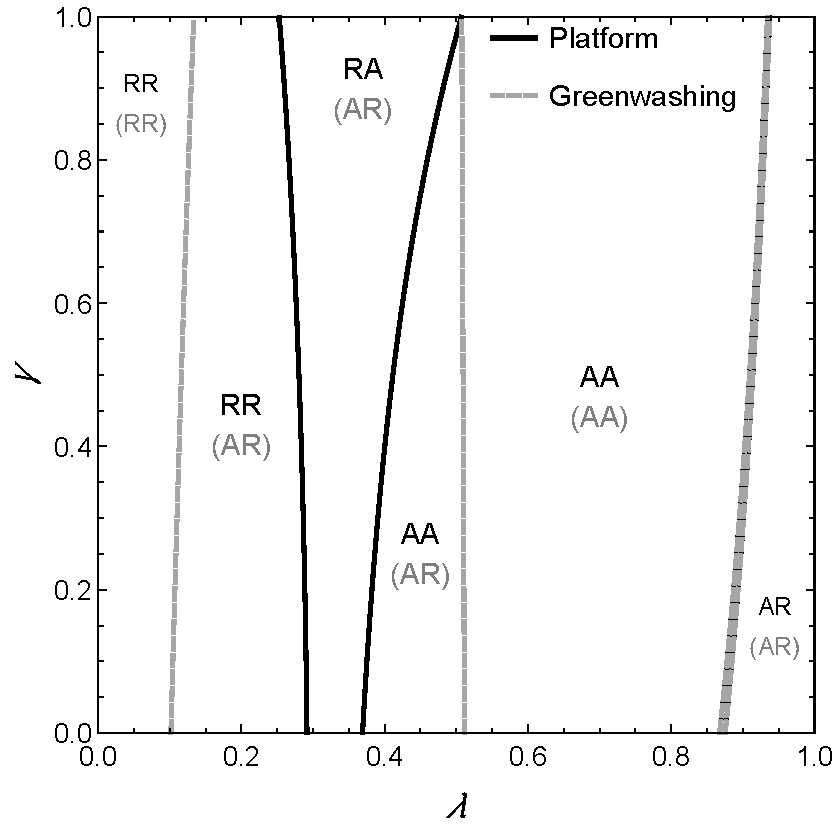
\includegraphics[width=0.55\textwidth]{duibi.pdf}
\caption{Platform-profit-maximizing and greenwashing-minimizing selling formats without blockchain ($a=1$, $b=0.2$, $\rho=0.3$, $\theta=1.4$, $k=0.4$, $g=0.3$).}
\label{fig:format-gw}
\end{figure}

Figure \ref{fig:format-gw} shows three regions that correspond closely to Proposition \ref{prop:ranking}. At low commissions (approximately $\lambda<0.1$ for the plotted parameters), the platform's profit objective and greenwashing control are aligned on RR; this is consistent with $\hat{\lambda}\in(0.102,0.134)$ across the plotted trust range. At intermediate commissions (roughly $0.1<\lambda<0.5$), AR minimizes greenwashing, whereas the platform may prefer RR, RA, or AA depending on consumer trust, so the two objectives diverge. At higher commissions they realign on AA and then AR. The final switch to AR at high commissions is a participation effect rather than a new greenwashing incentive: under agency the green supplier retains only $1-\lambda$ of revenue and can no longer cover the greenness cost, so AA becomes infeasible and the green product must return to reselling.

\subsection{Blockchain adoption scenario}

We now examine equilibrium outcomes under blockchain verification. The next lemma shows how the per-unit verification cost affects each member's profit across the four selling formats.

\begin{lemma}\label{lem:cost}
A higher blockchain cost $c_g$ affects profits as follows:\\
(1) The platform's profit decreases in RR, RA, and AA; in AR it can increase.\\
(2) The green supplier's profit decreases in RR, RA, and AR and is unaffected in AA.\\
(3) The ordinary supplier's profit increases in RR, RA, and AR and is unaffected in AA.
\end{lemma}

The platform-profit result in Lemma \ref{lem:cost}(1) has a distinct mechanism in AR. Because the ordinary product is sold by agency, a higher verification cost can shift demand toward it and increase the platform's commission revenue enough to raise its overall profit; Appendix B gives the exact condition. Specifically, a higher verification cost raises both retail prices but raises the green resale price more than the ordinary agency price, shifting demand toward the ordinary product and expanding the platform's commission base; the resulting increase in ordinary-product commissions can offset both the lost green resale margin and the verification cost. Verified greenness does not automatically translate into a higher green retail price: the green product commands a premium only if $g>\hat{g}^{Bj}$, a format-specific threshold derived in Appendix B. This threshold reflects the interaction of genuine greenness with who controls each retail price and the cross-price response between the two products; green demand must rise enough to overcome the price gap created by the selling formats.

\subsection{Comparison and optimal strategy}

\subsubsection{Joint choice of selling format and blockchain adoption}

For a fixed configuration $j$, the platform's adoption incentive is
\begin{equation*}
\Delta_p^j=\pi_p^{Bj}-\pi_p^{Nj}.
\end{equation*}
Blockchain restores trust, removes demand generated by exaggerated claims, and adds a verification cost. We characterize the adoption regions numerically here; Section \ref{sec:5} derives a common analytical trust threshold once greenness is endogenous.

Figure \ref{fig:platform} shows the platform's highest-profit choice of selling format and blockchain adoption at each commission rate and level of consumer trust. Shaded regions indicate blockchain adoption, and solid lines separate optimal selling formats.

\begin{figure}[t]
\centering
\subfloat[$g=0.3$]{\label{fig:platform-a}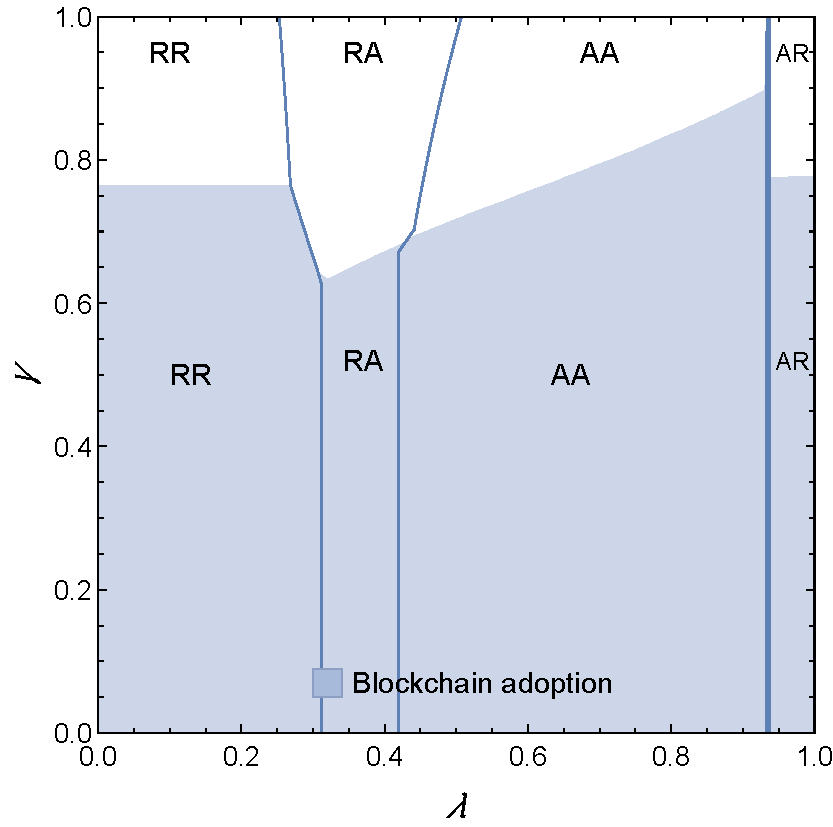
\includegraphics[width=0.47\textwidth]{Fig1a.pdf}}
\hfill
\subfloat[$g=0.6$]{\label{fig:platform-b}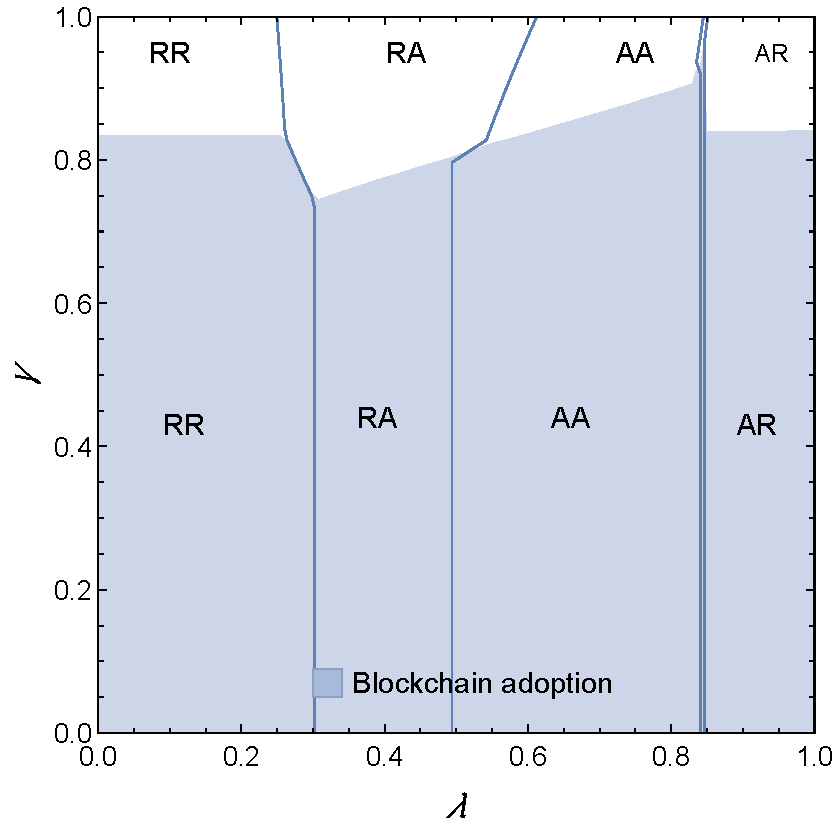
\includegraphics[width=0.47\textwidth]{Fig1b.pdf}}
\caption{Platform's optimal choice ($a=1$, $b=0.2$, $\rho=0.3$, $\theta=1.4$, $k=0.4$, $c_g=0.02$).}
\label{fig:platform}
\end{figure}

Figure \ref{fig:platform} shows two threshold patterns. First, blockchain is adopted at low trust and forgone at high trust. Across the two panels, the adoption boundary lies at approximately $\gamma=0.63$--$0.90$ for $g=0.3$ and $\gamma=0.74$--$0.91$ for $g=0.6$; its position varies with the commission rate. When trust is low, unverified claims are heavily discounted, so verified greenness generates enough additional demand to justify the verification cost; when trust is high, unverified claims already create substantial demand and verification mainly removes sales generated by exaggerated claims while adding cost. Second, the selling-format sequence is driven mainly by the commission rate: RR $\rightarrow$ RA $\rightarrow$ AA. At very high commissions, however, the green supplier's agency participation constraint makes AA infeasible. This creates the narrow RA band visible near the right edge of Figure \ref{fig:platform}: over this small interval the platform still keeps the ordinary product under reselling while the green product remains in agency, before the green supplier's participation constraint tightens further and the platform switches to AR, placing the green product back under reselling.

\subsubsection{Consumer surplus and welfare}

Following \citet{singh1984,liu2014ad,wu2015online}, let $D=(D_o,D_g)^\top$ and $M=\left(\begin{smallmatrix}1&-b\\-b&1\end{smallmatrix}\right)$. Inverse demand has slope $-M^{-1}$, so integrating it up to the quantities consumers choose and subtracting their expenditure gives surplus evaluated at the attributes they perceive:
\begin{equation}\label{eq:perceived-cs}
CS=\frac{1}{2}D^\top M^{-1}D
=\frac{D_o^2+2bD_oD_g+D_g^2}{2(1-b^2)}.
\end{equation}
Without verification, consumers base their purchases on $\gamma(1+\beta)g$ rather than true greenness $g$. Let $\delta=\gamma(1+\beta)g-g$ denote this perceived-minus-true gap. Holding the chosen quantities and expenditure fixed, evaluating utility at true greenness shifts the green demand intercept by $-\delta$ and changes surplus by $-\delta(M^{-1}D)_g=-\delta(D_g+bD_o)/(1-b^2)$. Realized consumer surplus is therefore
\begin{equation}\label{eq:realized-cs}
CS^{R}=CS-\frac{\delta\,(D_g+bD_o)}{1-b^2}.
\end{equation}
Under blockchain, $\delta=0$ and the two surplus measures coincide. For a fixed selling format $j$, write the adoption effect as $\Delta CS^{R,j}=CS^{Bj}-CS^{R,Nj}$. Figure \ref{fig:cs} compares perceived CS across configurations and the effect of blockchain adoption.

\begin{figure}[H]
\centering
\subfloat[Highest CS]{\label{fig:cs-a}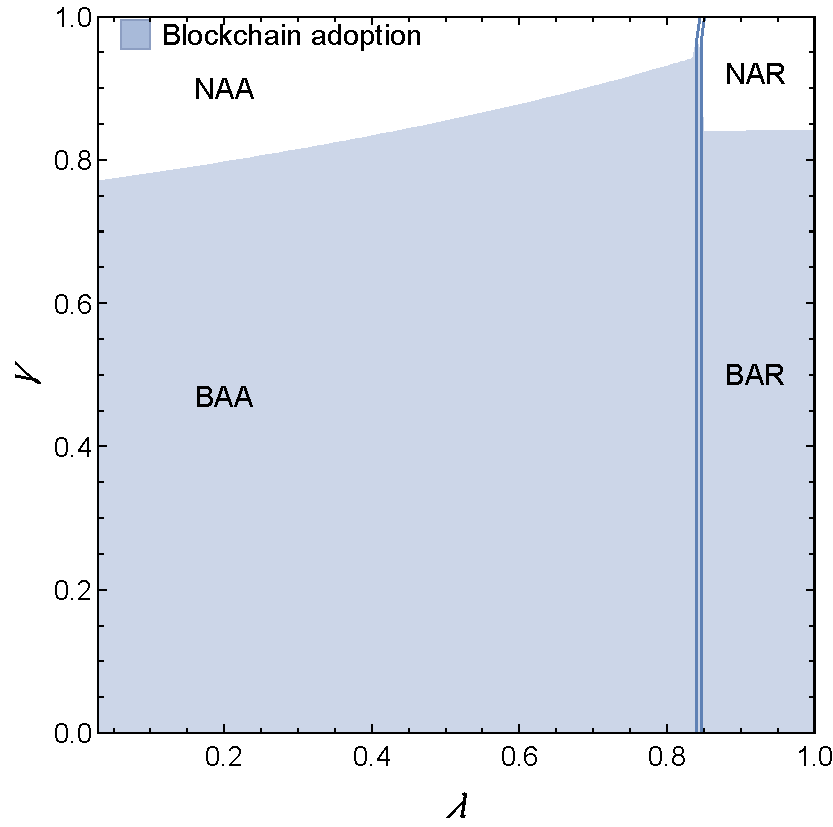
\includegraphics[width=0.47\textwidth]{CS1.pdf}}
\hfill
\subfloat[Blockchain effect]{\label{fig:cs-b}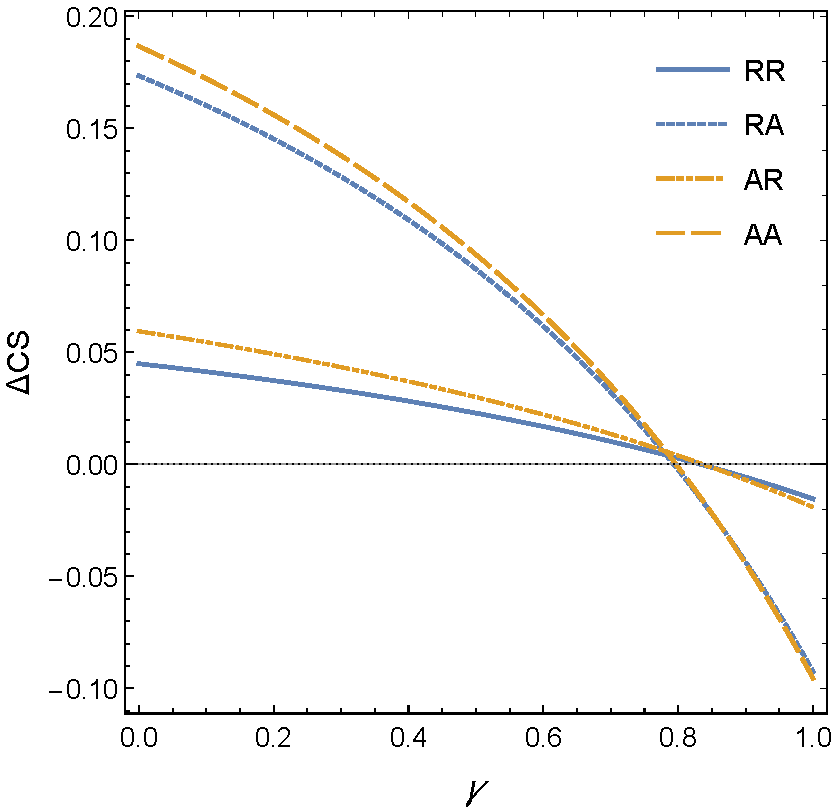
\includegraphics[width=0.47\textwidth]{CS2.pdf}}
\caption{Perceived consumer surplus ($a=1$, $b=0.2$, $\rho=0.3$, $\theta=1.4$, $k=0.4$, $c_g=0.02$, $g=0.6$; panel (b): $\lambda=0.2$).}
\label{fig:cs}
\end{figure}

Blockchain raises perceived CS when consumer trust is below about $0.8$ and lowers it when trust is higher, broadly mirroring the platform's adoption pattern. The effect is larger in RA and AA because the green supplier sets the retail price and can translate verified greenness directly into demand. Over most of the plotted region perceived CS is highest under BAA; at high trust, NAA can instead dominate because verification removes demand that consumers were willing to generate from the unverified claim.

\begin{proposition}\label{prop:realized}
Let $c_g=0$ and suppose both equilibria under configuration $j$ are feasible.\\
(1) If $\gamma(1+\beta^{Nj})>1$, then $\Delta CS^{R,j}>0$; if $\gamma(1+\beta^{Nj})=1$, then $\Delta CS^{R,j}=0$.\\
(2) If $\gamma(1+\beta^{Nj})<1$, then $\Delta CS^{R,j}<0$ if and only if $g-\gamma(1+\beta^{Nj})g<\bar{\delta}^j$, where $\bar{\delta}^j>0$ is given in Appendix B.
\end{proposition}

The sign of $\delta$ distinguishes overvaluation from undervaluation of true greenness. Verification raises realized consumer surplus when $\delta>0$; when $\delta<0$, it can lower surplus if the understatement is smaller than $\bar{\delta}^j$, while a larger correction can expand demand enough to reverse the effect.

To distinguish changes in efficiency from transfers between consumers and firms, define $W=CS^{R}+\pi_o+\pi_g+\pi_p$. Payments between members cancel, so $W$ equals consumers' utility at true greenness minus greenness, greenwashing, and verification costs.

\begin{proposition}\label{prop:welfare}
Let $c_g=0$ and suppose both equilibria under configuration $j$ are feasible. Let $\delta^j$ be the gap $\delta$ at the no-blockchain equilibrium under $j$, and let $d^j=\partial D^{Bj}/\partial g$, whose components are positive. Then
\begin{equation*}
\Delta W^j=W^{Bj}-W^{Nj}=\theta(\beta^{Nj}g)^2-\delta^j\,(d^j)^\top p^{Bj}+\tfrac12(\delta^j)^2(d^j)^\top M^{-1}d^j,
\end{equation*}
where $p^{Bj}=(p_o^{Bj},p_g^{Bj})^\top$. If $\gamma(1+\beta^{Nj})\leq1$, then $\Delta W^j>0$.
\end{proposition}

Proposition \ref{prop:welfare} separates the saved greenwashing cost from the effects of correcting beliefs and changing output. When claims understate true greenness, verification raises total welfare. When claims overstate it, verification can protect consumers yet lower welfare if removing claim-driven demand further reduces output under market power. Figure \ref{fig:cs-real} compares the consumer-surplus and welfare effects.

\begin{figure}[H]
\centering
\subfloat[Realized consumer surplus]{\label{fig:cs-real-a}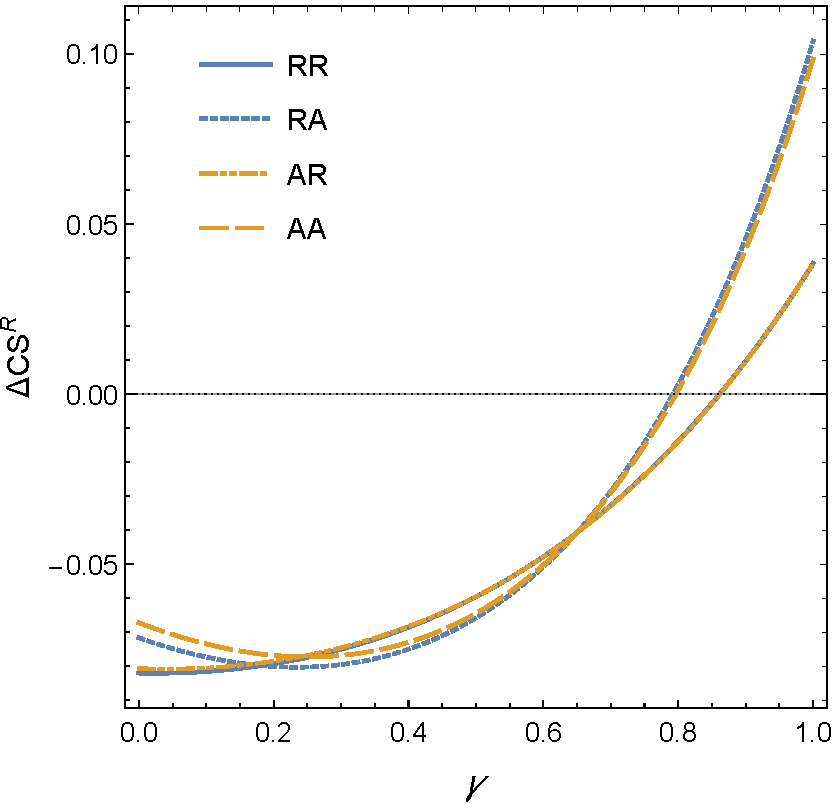
\includegraphics[width=0.47\textwidth]{CS3.pdf}}
\hfill
\subfloat[Total welfare]{\label{fig:cs-real-b}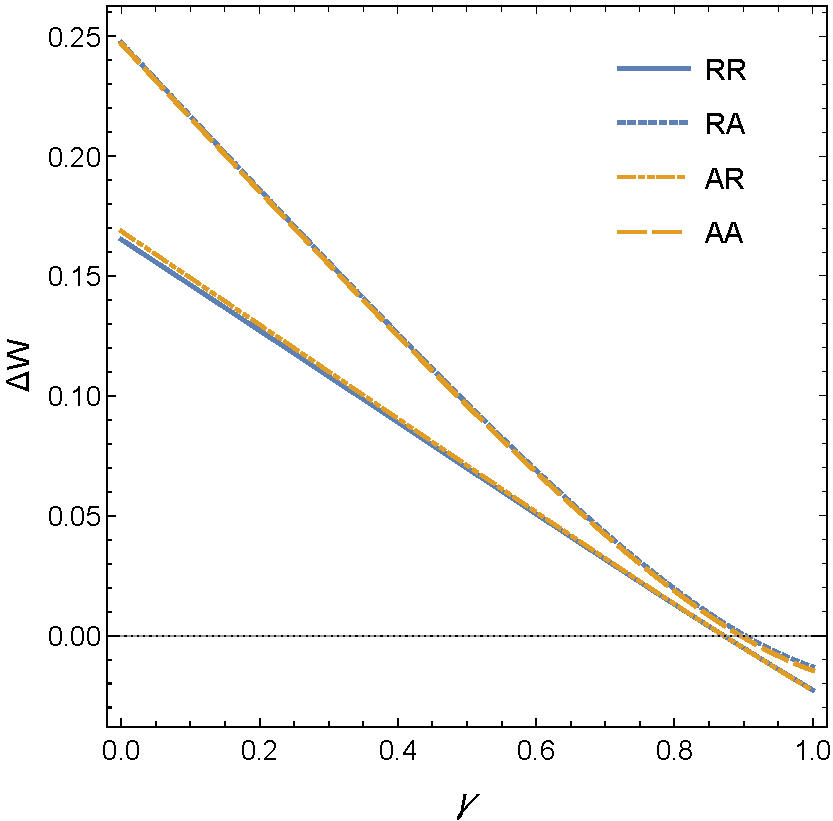
\includegraphics[width=0.47\textwidth]{W1.pdf}}
\caption{Effect of blockchain on realized consumer surplus and total welfare ($a=1$, $b=0.2$, $\rho=0.3$, $\theta=1.4$, $k=0.4$, $c_g=0.02$, $g=0.6$, $\lambda=0.2$).}
\label{fig:cs-real}
\end{figure}

In Figure \ref{fig:cs-real-a}, blockchain lowers realized CS at low trust because consumers otherwise obtain genuine greenness at discounted prices; at high trust, it raises CS by removing payments for greenness that is not delivered. The switch is close to $\delta=0$, with a small displacement due to the positive verification cost used in the figure.

Figure \ref{fig:cs-real-b} shows that, at $\lambda=0.2$, blockchain raises total welfare until roughly $\gamma=0.871$--$0.902$ across formats, while perceived greenness reaches true greenness earlier, around $\gamma=0.793$--$0.854$. In RR, which the platform selects at this commission rate, its adoption boundary in Figure \ref{fig:platform-b} lies at $\gamma\approx0.833$, the perceived and true greenness levels coincide at $\gamma\approx0.854$, and verification stops raising total welfare at $\gamma\approx0.871$. Thus, the platform can forgo verification while it still improves total welfare; the consumer-surplus threshold need not coincide with either boundary.

\section{Joint Decisions on Genuine Greenness and Exaggeration}\label{sec:5}

In the basic model, product greenness $g$ is exogenous and the green supplier chooses only the exaggeration level $\beta$. We now endogenize both environmental decisions. Without blockchain, the green supplier jointly chooses genuine greenness $g$ and the exaggeration level $\beta$ at Stage 1 together with his price term. With blockchain verification, exaggeration is eliminated ($\beta=0$), so the supplier chooses only genuine greenness. The timing, contract structure, and absolute-exaggeration cost $\theta(\beta g)^2$ are the same as in the basic model.

As in the basic model, $\beta\geq0$ is the proportion by which the supplier inflates true greenness: the claim is $(1+\beta)g$ and perceived greenness is $\gamma(1+\beta)g$. The cost $\theta(\beta g)^2$ continues to depend on the absolute exaggeration $\beta g$; now both $g$ and $\beta$ are choices. Without blockchain, the green product's demand and the green supplier's profit become
\begin{equation}\label{eq:ext}
D_g^{N}=(1-\rho)a-p_g+bp_o+\gamma(1+\beta)g,\qquad \pi_g^{Nj}=R_g^{j}-\frac{k}{2}g^2-\theta\beta^2g^2,
\end{equation}
where $R_g^{j}$ denotes the green supplier's revenue under configuration $j$ ($w_gD_g^N$ under reselling and $(1-\lambda)p_gD_g^N$ under agency).

\begin{lemma}\label{lem:endog-g}
When blockchain is adopted, the equilibrium greenness $g^{Bj}$ is positive if $k>\tilde{k}^{Bj}$ and $c_g<\tilde{c}_g^{Bj}$, where $\tilde{k}^{BRR}=\frac{1}{4-b^2}$, $\tilde{k}^{BRA}=\frac{4(1-\lambda)}{8-b^2(3\lambda+5)}$, $\tilde{k}^{BAR}=\frac{4-b^2(3\lambda+1)}{2(8-b^2(3\lambda+5))}$, and $\tilde{k}^{BAA}=\frac{2(1-\lambda)}{4-b^2}$. The cost thresholds $\tilde{c}_g^{Bj}$ are given in Appendix B; in BAA, no cost condition is needed.
\end{lemma}

The condition $k>\tilde{k}^{Bj}$ requires genuine greenness to be sufficiently costly relative to its demand effect. The basic-model value $k=0.4$ violates this condition in the agency formats at low commission rates (e.g., $\tilde{k}^{BAA}\approx0.5$ as $\lambda\to0$). Without blockchain, the analogous condition applies to the effective greenness-cost coefficient described in Proposition \ref{prop:equivalence}. The numerical analysis in this section therefore uses $k=1.2$, while retaining $\theta=1.4$ and all other parameter values.

\begin{proposition}\label{prop:greenness}
Under blockchain, suppose $\lambda\leq\frac12$, $k>\tilde{k}^{BRA}$, and all four configurations have interior equilibria. Then $g^{BRA}>\max\{g^{BRR},g^{BAR},g^{BAA}\}$ and $g^{BAA}\geq g^{BRR}$, so the lowest greenness is $\min\{g^{BRR},g^{BAR}\}$.
\end{proposition}

RA gives the green supplier direct pricing control while leaving most of his revenue with him when $\lambda\leq1/2$; the ordinary product's resale price also softens the green supplier's competitive response. This makes genuine investment attractive after verification. Proposition \ref{prop:equivalence}(4) shows that, without verification, RA also increases exaggeration. RA can therefore raise both genuine greenness and greenwashing. \citet{wuZhao2027cooperative} find that reselling can outperform agency for greenness at higher commissions under green R\&D cost sharing.

Without blockchain, the green supplier chooses genuine greenness and exaggeration jointly. The following proposition characterizes this choice analytically.

\begin{proposition}\label{prop:equivalence}
Suppose the no-blockchain game with endogenous greenness has an interior equilibrium under configuration $j$.\\
(1) $\beta^{Nj}=k/(2\theta)$ for every $j$.\\
(2) Equilibrium prices, demands, and profits coincide with those of the blockchain game with $c_g=0$ when its greenness-cost parameter is set to $\frac{2k\theta}{(k+2\theta)\gamma^2}$. In this equivalent blockchain game, equilibrium greenness equals $\gamma(1+\beta^{Nj})g^{Nj}$.\\
(3) If $c_g=0$ and both equilibria are feasible, every member strictly prefers blockchain adoption if and only if $\gamma<\hat{\gamma}\equiv\sqrt{2\theta/(k+2\theta)}$.\\
(4) If $\lambda\leq\frac12$ and Proposition \ref{prop:greenness} applies to the blockchain game with $c_g=0$ and greenness-cost parameter $\frac{2k\theta}{(k+2\theta)\gamma^2}$, then RA yields the highest $g^{Nj}$ and the highest absolute exaggeration $\beta^{Nj}g^{Nj}$.
\end{proposition}

Proposition \ref{prop:equivalence} characterizes the green supplier's two environmental decisions. Genuine greenness $g$ improves the product itself, while exaggeration $\beta$ raises reported greenness without changing the product. Because both raise perceived greenness in the unverified market, the first-order conditions give $\beta=k/(2\theta)$ in every selling format. Relative costs therefore determine proportional exaggeration. Selling format and consumer trust determine equilibrium genuine greenness and, through it, the absolute amount exaggerated $\beta g$. A contract that raises genuine greenness can therefore also increase greenwashing. Higher genuine greenness and lower greenwashing are not the same outcome.

Part (2) gives a useful equivalence. Exaggeration lowers the cost of creating perceived greenness, while consumer distrust reduces its market value. In the model, these two effects can be summarized by an adjusted greenness cost. With costless verification, this leads to the same adoption threshold for the platform and both suppliers in every selling format. A positive verification cost lowers the platform's threshold, as Figure \ref{fig:endog-choice} shows. Selling contracts determine how much genuine greenness is chosen and how much is exaggerated; verification removes exaggeration from the supplier's choice.

The same logic extends when consumers put different weights on genuine greenness and exaggeration. If genuine greenness is partly verifiable, consumers can place more weight on genuine performance than on an exaggerated claim. The first-order conditions still give a proportional exaggeration that is independent of selling format, and the unverified game can still be written as a verified game with an adjusted greenness cost. The result changes when greenwashing costs depend on sales, for example when fines rise with the quantity sold under a false claim, or when the platform bears a reputational cost. In those cases, the selling format affects exaggeration through equilibrium sales as well as through genuine greenness.

Figures \ref{fig:endog-choice} and \ref{fig:endog-eg} illustrate these results. In Figure \ref{fig:endog-choice}, shading marks blockchain adoption, solid lines separate selling formats, and the dotted line marks the costless-verification threshold $\hat{\gamma}$. The shaded adoption boundary lies below $\hat{\gamma}$ because the figure uses a positive verification cost, $c_g=0.02$: costless verification would be attractive up to the common analytical threshold, whereas a positive cost requires a larger trust deficit before adoption becomes profitable. The small kinks in the adoption boundary occur where the platform's preferred selling format changes, because the profit effect of verification is evaluated under a different contract on each side of those boundaries.

\begin{figure}[t]
\centering
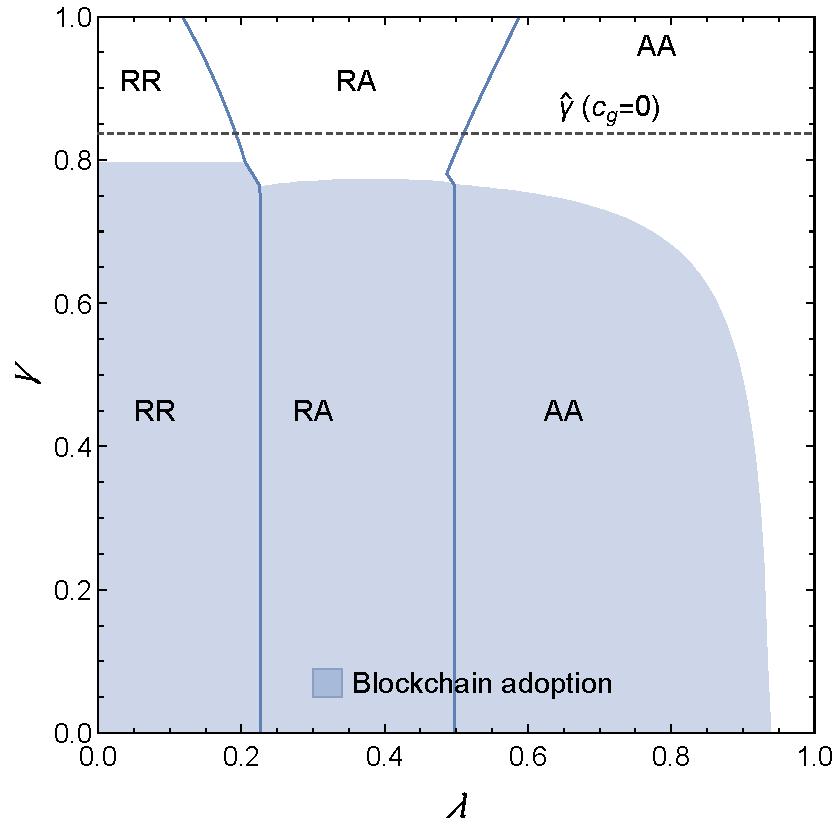
\includegraphics[width=0.55\textwidth]{Fig2.pdf}
\caption{Endogenous greenness: selling format and blockchain adoption ($a=1$, $b=0.2$, $\rho=0.3$, $\theta=1.4$, $k=1.2$, $c_g=0.02$).}
\label{fig:endog-choice}
\end{figure}

\begin{figure}[t]
\centering
\subfloat[Absolute exaggeration $\beta g$]{\label{fig:endog-beta}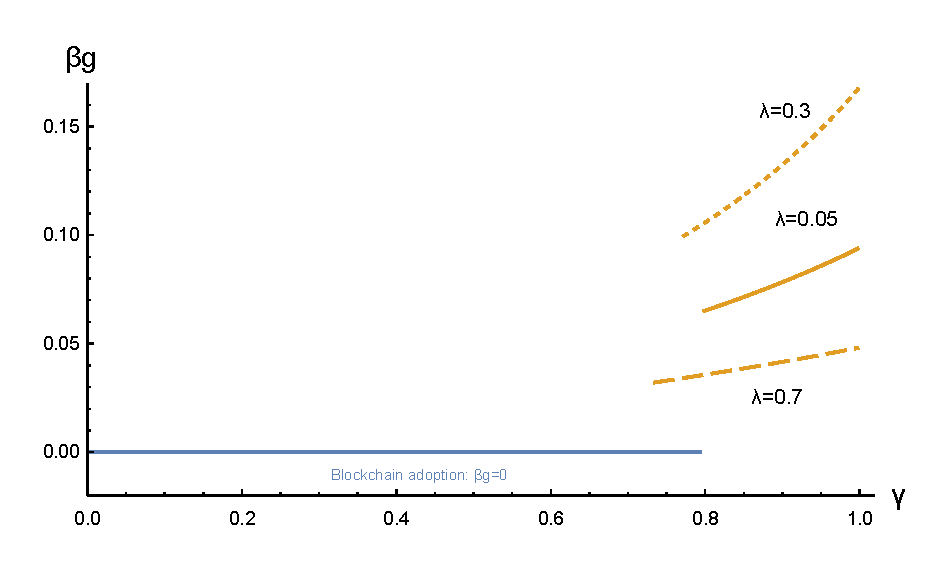
\includegraphics[width=0.47\textwidth]{fig51.pdf}}
\hfill
\subfloat[Greenness $g$]{\label{fig:endog-g}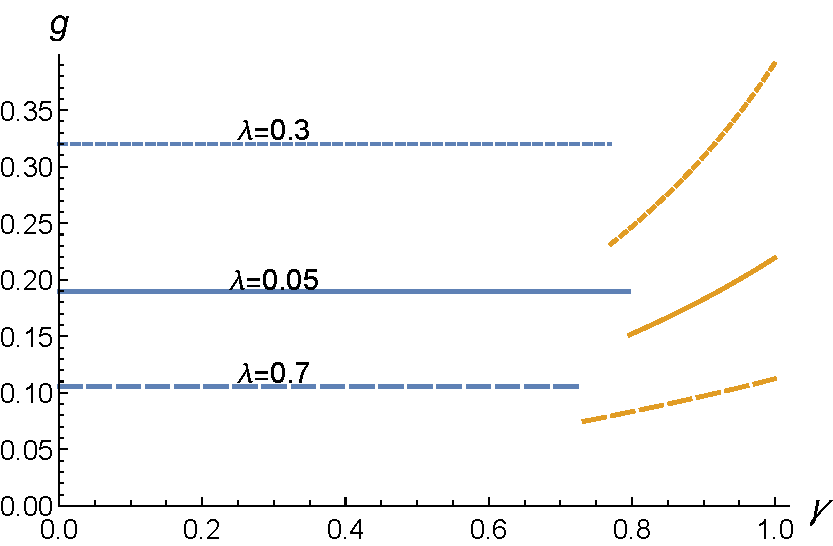
\includegraphics[width=0.47\textwidth]{fig52.pdf}}
\caption{Exaggeration and greenness ($a=1$, $b=0.2$, $\rho=0.3$, $\theta=1.4$, $k=1.2$, $c_g=0.02$; $\lambda=0.05,0.3,0.7$).}
\label{fig:endog-eg}
\end{figure}

Figure \ref{fig:endog-eg} reports endogenous greenness and absolute exaggeration under the platform's optimal strategy as consumer trust $\gamma$ varies. The commission rate is common across selling formats. We plot $\lambda=0.05$, $0.3$, and $0.7$ as representative cases with low, intermediate, and high commission rates, in which the platform's preferred format is RR, RA, and AA, respectively. At each trust level, the platform's selling format and blockchain decision are optimized jointly. In panel (a), the zero-exaggeration line under blockchain is omitted; panel (b) shows the corresponding blue blockchain-adoption segments. Orange curves indicate no adoption. Under blockchain (low trust), exaggeration is zero and genuine greenness does not depend on $\gamma$. Once trust is high enough that the platform forgoes blockchain, genuine greenness drops discretely, because the supplier substitutes exaggeration for part of his genuine investment. Both $\beta g$ and $g$ then rise with $\gamma$, while the inflation ratio remains $\beta=k/(2\theta)\approx0.429$, as Proposition \ref{prop:equivalence} predicts. These curves use different commission rates to illustrate the platform's selected strategy and do not establish a cross-format ranking at a common commission. For a like-for-like comparison at $\lambda=0.3$ and $\gamma=0.9$, no-blockchain greenness is $g^{NRA}=0.309>g^{NAA}=0.294>g^{NRR}=0.183>g^{NAR}=0.181$; Proposition \ref{prop:equivalence}(4) then implies the same ordering for absolute exaggeration.

\section{Conclusions and Managerial Implications}\label{sec:6}

\subsection{Summary of findings}

We analyze how platform selling formats and verification affect greenwashing in a supply chain with competing ordinary and green suppliers. The platform chooses one of four selling-format configurations and whether to adopt blockchain verification. We first hold true greenness fixed, then let the green supplier choose both genuine greenness and exaggeration.

The format determines how pricing authority and revenue sharing translate inflated claims into supplier profit. RA never minimizes greenwashing and is the most greenwashing-intensive format when the commission is at most one half. At low commissions, RR or AR can instead minimize it; at higher commissions, AA or AR can be least greenwashing, depending on feasibility and parameters. The format that maximizes platform profit need not minimize exaggeration.

Verification has two effects: it makes true greenness observable and removes demand induced by exaggerated claims. Consequently, consumer protection, platform profit, and total welfare need not move together. When consumers' unverified perception falls below true greenness, verification can reduce realized consumer surplus; when claims overstate true performance, it can raise realized consumer surplus. Total welfare also depends on how verification changes output under market power. For the plotted parameter values, blockchain raises welfare up to trust levels that can exceed the platform's adoption boundary, so a platform may forgo a welfare-improving verification system.

When the green supplier chooses greenness and exaggeration jointly, the equilibrium proportional exaggeration is $\beta=k/(2\theta)$ in every selling format. Contract structure and consumer trust affect genuine greenness and therefore the absolute amount exaggerated. For example, at $\lambda=0.3$ and $\gamma=0.9$, the no-blockchain greenness ordering is RA ($0.309$), AA ($0.294$), RR ($0.183$), and AR ($0.181$). Thus, greater genuine greenness can coincide with greater absolute greenwashing. With costless verification, every supply chain member prefers adoption if and only if $\gamma<\sqrt{2\theta/(k+2\theta)}$.

\subsection{Managerial implications}

\textbf{For platform managers.} Evaluate selling formats on at least three dimensions: platform profit, genuine greenness, and exaggeration. A format that supports green investment may also raise the supplier's return from inflated claims. Verification is most valuable when unverified claims are heavily discounted, but the platform's private adoption incentive can fall short of the welfare-improving range. Managers should therefore report the consumer and welfare effects alongside the profit calculation.

\textbf{For green suppliers.} Agency selling combines direct pricing control with a commission paid to the platform. Its effect on environmental choices depends on the format assigned to the competing ordinary product and on consumer trust. In the model, low trust increases the value of credible verification; when verification is costless, the supplier prefers it below the common threshold stated in Proposition \ref{prop:equivalence}.

\textbf{For policymakers and regulators.} Higher genuine investment does not by itself show that misleading claims have declined. Disclosure and traceability rules should distinguish true environmental performance from the claims made about it. Evaluation should also separate realized consumer surplus from total welfare, since verification can improve one while reducing the other.

\subsection{Limitations and future research}

The model treats consumer trust $\gamma$ as an exogenous reduced-form belief. Consumers do not infer the supplier's equilibrium exaggeration from the fact that a claim is unverified; this captures limited information or stable prior beliefs. Allowing trust to update with observed claims, past verification, or disclosure could change both demand and the platform's adoption threshold. Other extensions include endogenous or supplier-specific commissions, competing platforms, imperfect verification, fixed adoption costs, environmental damages, and greenwashing penalties that depend on sales. Empirical work could test the model once transaction-level platform data can be linked to credible measures of true environmental performance.

%% ============================================================
\appendix
\section{Optimal decisions and profits}\label{app:A}
\begingroup\small

For the four no-blockchain cases below, write $\vartheta=\theta g^2$. These are the fixed-$g$ equilibrium expressions with the absolute-exaggeration cost coefficient substituted exactly.

\noindent\textit{Case NRR}\\
$w_g^{NRR}=\frac{2 \vartheta  (a (2-(2-b) \rho )+2 \gamma  g)}{2 \left(4-b^2\right) \vartheta -\gamma ^2 g^2}$,
$w_o^{NRR}=\frac{a \rho  \left(\gamma ^2 g^2-4 (2-b) \vartheta \right)-4 b \vartheta  (a+\gamma  g)}{2 \gamma ^2 g^2-4 \left(4-b^2\right) \vartheta }$,
$\beta^{NRR}=\frac{\gamma  g (a (2-(2-b) \rho )+2 \gamma  g)}{4 \left(4-b^2\right) \vartheta -2 \gamma ^2 g^2}$,\\
$p_g^{NRR}=\frac{a \rho  \left(b \gamma ^2 g^2+4 (1-b) (2-b) (2 b+3) \vartheta \right)-12 \left(2-b^2\right) \vartheta  (a+\gamma  g)}{4 \left(1-b^2\right) \left(\gamma ^2 g^2-2 \left(4-b^2\right) \vartheta \right)}$,\\
$p_o^{NRR}=\frac{a \rho  \left(\left(2 b^2-3\right) \gamma ^2 g^2+4 (1-b) (2-b) (2 b+3) \vartheta \right)+4 b \left(5-2 b^2\right) \vartheta  (a+\gamma  g)}{4 \left(1-b^2\right) \left(2 \left(4-b^2\right) \vartheta -\gamma ^2 g^2\right)}$,\\
$\pi_g^{NRR}=\frac{\vartheta  \left(8 \vartheta -\gamma ^2 g^2\right) (a (2-(2-b) \rho )+2 \gamma  g)^2-2 k \left(\gamma ^2 g^3-2 \left(4-b^2\right) g \vartheta \right)^2}{4 \left(\gamma ^2 g^2-2 \left(4-b^2\right) \vartheta \right)^2}$,
$\pi_o^{NRR}=\frac{\left(4 b \vartheta  (a+\gamma  g)-a \rho  \left(\gamma ^2 g^2-4 (2-b) \vartheta \right)\right)^2}{8 \left(\gamma ^2 g^2-2 \left(4-b^2\right) \vartheta \right)^2}$,\\
$\pi_p^{NRR}=\frac{a^2 \rho ^2 \left(\gamma ^4 g^4-8 (2-b) (1-b) \gamma ^2 g^2 \vartheta +32 (1-b) (2-b)^2 \vartheta ^2\right)+16 \left(5 b^2+4\right) \vartheta ^2 (a+\gamma  g)^2-8 a \vartheta  \rho  (a+\gamma  g) \left(3 b \gamma ^2 g^2+4 (1-b) (2-b)^2 \vartheta \right)}{16 \left(1-b^2\right) \left(\gamma ^2 g^2-2 \left(4-b^2\right) \vartheta \right)^2}$.

\vspace{0.3cm}
\noindent\textit{Case NRA}\\
$w_o^{NRA}=\frac{a \rho  \left(4 \vartheta-b \vartheta  (3 b \lambda +b-2 \lambda +2)-\gamma ^2 g^2 (1-\lambda )\right)+2 b \vartheta  (1-\lambda ) (a+\gamma  g)}{\vartheta  \left(8-b^2 (3 \lambda +5)\right)-2 \gamma ^2 g^2 (1-\lambda )}$,
$\beta^{NRA}=\frac{\gamma  g (1-\lambda ) (a (4-(4-3 b) \rho )+4 \gamma  g)}{2 \vartheta  \left(8-b^2 (3 \lambda +5)\right)-4 \gamma ^2 g^2 (1-\lambda )}$, \\
$p_g^{NRA}=\frac{\vartheta  (a (4-(4-3 b) \rho )+4 \gamma  g)}{\vartheta  \left(8-b^2 (3 \lambda +5)\right)-2 \gamma ^2 g^2 (1-\lambda )}$,
$p_o^{NRA}=\frac{a \vartheta  \rho  \left(12-3 b^2 (\lambda +1)-2 b (\lambda +3)\right)+2 b \vartheta  (\lambda +3) (a+\gamma  g)-3 a \gamma ^2 g^2 (1-\lambda ) \rho }{2 \vartheta  \left(8-b^2 (3 \lambda +5)\right)-4 \gamma ^2 g^2 (1-\lambda )}$,\\
$\pi_g^{NRA}=\frac{\vartheta  (1-\lambda ) (a (4-(4-3 b) \rho )+4 \gamma  g)^2 \left(4 \vartheta-2 b^2 \vartheta  (\lambda +1)-\gamma ^2 g^2 (1-\lambda ) \right)}{4 \left(2 \gamma ^2 g^2 (1-\lambda )-\vartheta  \left(8-b^2 (3 \lambda +5)\right)\right)^2}-\frac{g^2 k}{2}$,\\
$\pi_o^{NRA}=\frac{\left(a \rho  \left(\vartheta  (b (3 b \lambda +b-2 \lambda +2)-4)+\gamma ^2 g^2 (1-\lambda )\right)-2 b \vartheta  (1-\lambda ) (a+\gamma  g)\right)^2}{2 \left(2 \gamma ^2 g^2 (1-\lambda )-\vartheta  \left(8-b^2 (3 \lambda +5)\right)\right)^2}$,\\
$\pi_p^{NRA}=\frac{1}{4 (\vartheta  \left(8-b^2 (3 \lambda +5)\right)-2 \gamma ^2 g^2 (1-\lambda ))^2}[4 \gamma ^2 g^2 \vartheta ^2 (b^2 (1-\lambda  (11 \lambda +6))+16 \lambda )-4 a \gamma  g \vartheta  (b^3 \vartheta  (\lambda  (18 \lambda +13)+1) \rho -2 b^2 \vartheta  (1-\lambda  (11 \lambda +6)) (1-\rho )-b \rho  (4 (7 \vartheta  \lambda +\vartheta )-\gamma ^2 g^2 (1-\lambda ^2))+32 \vartheta  \lambda  (\rho -1))+a^2 (b^4 \vartheta ^2 (1-9 \lambda  (3 \lambda +2)) \rho ^2+4 b^3 \vartheta ^2 (\lambda  (18 \lambda +13)+1) (\rho -1) \rho +2 b^2 \vartheta  (\gamma ^2 g^2 (1-\lambda ) \rho ^2-2 \vartheta  (11 \lambda ^2 (1-\rho )^2-3 \lambda  \rho  (\rho +4)+6 \lambda +\rho  (\rho +2)-1))+4 b \vartheta  (1-\rho ) \rho  (4 (7 \vartheta  \lambda +\vartheta )-\gamma ^2 g^2 (1-\lambda ^2))+\gamma ^4 g^4 (1-\lambda )^2 \rho ^2-8 \gamma ^2 g^2 \vartheta  (1-\lambda ) \rho ^2+16 \vartheta ^2 (4 \lambda  (1-\rho )^2+\rho ^2))]$.

\vspace{0.3cm}
\noindent\textit{Case NAR}\\
$w_g^{NAR}=\frac{4 \vartheta  \left(4-b^2 (3 \lambda +1)\right) (a+\gamma  g)-4 a \vartheta  \rho  (4-b (3 b \lambda +b-2 \lambda +2))}{4 \vartheta  \left(8-b^2 (3 \lambda +5)\right)-\gamma ^2 g^2 \left(4-b^2 (3 \lambda +1)\right)}$,\\
$\beta^{NAR}=\frac{\gamma  g \left(\left(4-b^2 (3 \lambda +1)\right) (a+\gamma  g)-a \rho  (4-b (3 b \lambda +b-2 \lambda +2))\right)}{4 \vartheta  \left(8-b^2 (3 \lambda +5)\right)-\gamma ^2 g^2 \left(4-b^2 (3 \lambda +1)\right)}$, \\
$p_g^{NAR}=\frac{6 \vartheta  \left(4-b^2 (\lambda +1)\right) (a+\gamma  g)+2 a \rho  \left(b (3 b+2) \vartheta  \lambda -b \gamma ^2 g^2 \lambda +3 (b (b+2)-4) \vartheta \right)}{4 \vartheta  \left(8-b^2 (3 \lambda +5)\right)-\gamma ^2 g^2 \left(4-b^2 (3 \lambda +1)\right)}$, \\
$p_o^{NAR}=\frac{12 b \vartheta  (a+\gamma  g)-2 a \rho  \left(6 b \vartheta +\gamma ^2 g^2-8 \vartheta \right)}{4 \vartheta  \left(8-b^2 (3 \lambda +5)\right)-\gamma ^2 g^2 \left(4-b^2 (3 \lambda +1)\right)}$, \\
$\pi_g^{NAR}=\frac{\left(8 \vartheta -\gamma ^2 g^2\right)\left(w_g^{NAR}\right)^2}{16\vartheta}-\frac{g^2 k}{2}$, \\
$\pi_o^{NAR}=\frac{2 (1-\lambda ) \left(2-b^2 (\lambda +1)\right) \left(a \rho  \left(6 b \vartheta +\gamma ^2 g^2-8 \vartheta \right)-6 b \vartheta  (a+\gamma  g)\right)^2}{(\gamma ^2 g^2 (b^2 (3 \lambda +1)-4)+4 \vartheta  (8-b^2 (3 \lambda +5)))^2}$, \\
$\pi_p^{NAR}=\frac{1}{\left(\gamma ^2 g^2 \left(b^2 (3 \lambda +1)-4\right)+4 \vartheta  (8-b^2 (3 \lambda +5)\right))^2}[-2 a^2 (\gamma ^4 g^4 \lambda  \rho ^2 (b^2 (\lambda +1)-2)+2 \gamma ^2 g^2 \vartheta  \lambda  \rho  (-(b^3 (9 \lambda +7) (1-\rho ))-2 b^2 (5 \lambda +3) \rho +16 b (1-\rho )+16 \rho )+2 \vartheta ^2 (b^4 (9 \lambda  (3 \lambda +2)-1) (1-\rho )^2-4 b^3 (\lambda  (18 \lambda +13)+1) (\rho -1) \rho +4 b^2 (11 \lambda ^2 \rho ^2-3 \lambda  (3-(6-\rho ) \rho )-(4-\rho ) \rho +2)-16 b (7 \lambda +1) (1-\rho ) \rho -16 (\rho  (4 \lambda  \rho +\rho -2)+1)))+4 a \gamma  g \vartheta  (b \gamma ^2 g^2 \lambda  \rho  (b^2 (9 \lambda +7)-16)+2 \vartheta (-(b^4 (9 \lambda  (3 \lambda +2)-1) (1-\rho ))-2 b^3 (\lambda  (18 \lambda +13)+1) \rho -4 b^2 (2-9 \lambda ) (1-\rho )+8 b (7 \lambda  \rho +\rho )+16 (1-\rho )))+4 \gamma ^2 g^2 \vartheta ^2 (b^4 (1-9 \lambda  (3 \lambda +2))-b^2 (8-36 \lambda )+16)]$.

\vspace{0.3cm}
\noindent\textit{Case NAA}\\
$\beta^{NAA}=\frac{\gamma  g (1-\lambda ) (a (2-(2-b) \rho )+2 \gamma  g)}{2 \left(4-b^2\right) \vartheta -2 \gamma ^2 g^2 (1-\lambda )}$,
$p_g^{NAA}=\frac{\vartheta  (a (2-(2-b) \rho )+2 \gamma  g)}{\left(4-b^2\right) \vartheta -\gamma ^2 g^2 (1-\lambda )}$,
$p_o^{NAA}=\frac{a \rho  \left(2 (2-b) \vartheta -\gamma ^2 g^2 (1-\lambda )\right)+2 b \vartheta  (a+\gamma  g)}{2 \left(4-b^2\right) \vartheta -2 \gamma ^2 g^2 (1-\lambda )}$,\\
$\pi_g^{NAA}=\frac{\vartheta  (1-\lambda ) \left(4 \vartheta -\gamma ^2 g^2 (1-\lambda )\right) (a (2-(2-b) \rho )+2 \gamma  g)^2}{4 \left(\gamma ^2 g^2 (1-\lambda )-\left(4-b^2\right) \vartheta \right)^2}-\frac{g^2 k}{2}$,
$\pi_o^{NAA}=\frac{(1-\lambda ) \left(a \rho  \left(2 (2-b) \vartheta -\gamma ^2 g^2 (1-\lambda )\right)+2 b \vartheta  (a+\gamma  g)\right)^2}{4 \left(\gamma ^2 g^2 (1-\lambda )-\left(4-b^2\right) \vartheta \right)^2}$,\\
$\pi_p^{NAA}=\frac{\lambda}{4 \left(\gamma ^2 g^2 (1-\lambda )-\left(4-b^2\right) \vartheta \right)^2}[a^2 (4 \vartheta ^2 \left(b^2+2 (2-b)^2 \rho ^2-2 (2-b)^2 \rho +4\right)-4 \gamma ^2 g^2 \vartheta  (1-\lambda ) \rho  ((2-b) \rho +b)+\gamma ^4 g^4 (1-\lambda )^2 \rho ^2)+4 a \gamma  g \vartheta  \left(2 \vartheta  \left(b^2+(2-b)^2 (-\rho )+4\right)+b \gamma ^2 g^2 (\lambda -1) \rho \right)+4 \left(b^2+4\right) \gamma ^2 g^2 \vartheta ^2]$.

\vspace{0.3cm}
\noindent\textit{Case BRR}\\
$w_g^{BRR}=\frac{2 (a+g)-a (2-b) \rho -\left(2-b^2\right) c_g}{4-b^2}$,
$w_o^{BRR}=\frac{b (a+g)+a (2-b) \rho +b c_g}{4-b^2}$,\\
$p_g^{BRR}=\frac{3 \left(2-b^2\right) (a+g)-a (2-b) (1-b) (2 b+3) \rho +2 \left(1-b^2\right) c_g}{2 \left(b^4-5 b^2+4\right)}$,
$p_o^{BRR}=\frac{b \left(5-2 b^2\right) (a+g)+a (1-b) (2-b) (2 b+3) \rho +\left(b-b^3\right) c_g}{2 \left(b^4-5 b^2+4\right)}$,\\
$\pi_g^{BRR}=\frac{a^2 (2-(2-b) \rho )^2-\left(2-b^2\right) c_g \left(-2 a (2-b) \rho +4 (a+g)-\left(2-b^2\right) c_g\right)+4 a g (2-(2-b) \rho )+g^2 \left(4-\left(4-b^2\right)^2 k\right)}{2 \left(4-b^2\right)^2}$,\\
$\pi_o^{BRR}=\frac{\left(b (a+g)+a (2-b) \rho +b c_g\right){}^2}{2 \left(4-b^2\right)^2}$,\\
$\pi_p^{BRR}=\frac{2 a^2 (1-b) (2-b)^2 \rho ^2+\left(1-b^2\right) c_g \left(-2 \left(b^2+4\right) (a+g)+2 a (2-b)^2 \rho +\left(4-3 b^2\right) c_g\right)+\left(5 b^2+4\right) (a+g)^2-2 a (1-b) (2-b)^2 \rho  (a+g)}{4 \left(4-b^2\right)^2 \left(1-b^2\right)}$.

\vspace{0.3cm}
\noindent\textit{Case BRA}\\
$w_o^{BRA}=\frac{2 b (1-\lambda ) (a+g)+a \rho  (4-b (3 b \lambda +b-2 \lambda +2))+b \left(4-b^2 (\lambda +3)\right) c_g}{8-b^2 (3 \lambda +5)}$,
$p_g^{BRA}=\frac{4 (a+g)-a (4-3 b) \rho-b^2 c_g}{8-b^2 (3 \lambda +5)}$,\\
$p_o^{BRA}=\frac{a \rho  \left(-3 b^2 (\lambda +1)-2 b (\lambda +3)+12\right)+2 b (\lambda +3) (a+g)-b \left(4-b^2 (\lambda +1)\right) c_g}{2 \left(8-b^2 (3 \lambda +5)\right)}$,\\
$\pi_g^{BRA}=\frac{1}{2} \left(\frac{(1-\lambda ) \left(2-b^2 (\lambda +1)\right) \left(a (4-3 b) \rho -4 (a+g)+b^2 c_g\right){}^2}{\left(8-b^2 (3 \lambda +5)\right)^2}-g^2 k\right)$,\\
$\pi_o^{BRA}=\frac{\left(a \rho  (b (3 b \lambda +b-2 \lambda +2)-4)-2 b (1-\lambda ) (a+g)-b \left(4-b^2 (\lambda +3)\right) c_g\right){}^2}{2 \left(8-b^2 (3 \lambda +5)\right)^2}$,\\
$\pi_p^{BRA}=\frac{1}{4 \left(8-b^2 (3 \lambda +5)\right)^2}[2 (2-b^2 (\lambda +1)) (-a (4-3 b) \rho +4 (a+g)+b^2 \left(-c_g\right)) (-a (4-3 b) \lambda  \rho +4 \lambda  (a+g)-\left(8-b^2 (2 \lambda +5)\right) c_g)-(2 b (\lambda -1) (a+g)+a \rho  (b (3 b \lambda +b-2 \lambda +2)-4)-b \left(4-b^2 (\lambda +3)\right) c_g) (2 b (3 \lambda +1) (a+g)+a \rho  (-3 (2-b) b \lambda -b (b+2)+4)-b \left(12-b^2 (3 \lambda +7)\right) c_g)]$.

\vspace{0.3cm}
\noindent\textit{Case BAR}\\
$w_g^{BAR}=\frac{(a+g) \left(4-b^2 (3 \lambda +1)\right)-a \rho  (4-b (3 b \lambda +b-2 \lambda +2))-\left(4-b^2 (\lambda +3)\right) c_g}{8-b^2 (3 \lambda +5)}$,\\
$p_g^{BAR}=\frac{3 (a+g) \left(4-b^2 (\lambda +1)\right)-a \rho  \left(12-3 b^2 (\lambda +1)-2 b (\lambda +3)\right)+\left(4-b^2 (\lambda +1)\right) c_g}{2 \left(8-b^2 (3 \lambda +5)\right)}$,
$p_o^{BAR}=\frac{3 b (a+g)+a (4-3 b) \rho +b c_g}{8-b^2 (3 \lambda +5)}$,\\
$\pi_g^{BAR}=\frac{1}{2} \left(\frac{\left((a+g) \left(4-b^2 (3 \lambda +1)\right)-a \rho  (4-b (3 b \lambda +b-2 \lambda +2))-\left(4-b^2 (\lambda +3)\right) c_g\right){}^2}{\left(8-b^2 (3 \lambda +5)\right)^2}-g^2 k\right)$,\\
$\pi_o^{BAR}=\frac{(1-\lambda ) \left(2-b^2 (\lambda +1)\right) \left(3 b (a+g)+a (4-3 b) \rho +b c_g\right){}^2}{2 \left(8-b^2 (3 \lambda +5)\right)^2}$,\\
$\pi_p^{BAR}=\frac{1}{4 \left(8-b^2 (3 \lambda +5)\right)^2}[2 \lambda  (2-b^2 (\lambda +1)) (3 b (a+g)+a (4-3 b) \rho +b c_g){}^2+\left((a+g) (b^2 (3 \lambda -1)+4\right)-a \rho  (-3 (2-b) b \lambda -b (b+2)+4)-(4-3 b^2 (\lambda +1)) c_g) ((a+g) (4-b^2 (3 \lambda +1))-a \rho  (4-b (3 b \lambda +b-2 \lambda +2))-\left(4-b^2 (\lambda +3)\right) c_g)]$.

\vspace{0.3cm}
\noindent\textit{Case BAA}\\
$p_g^{BAA}=\frac{2 (a+g)-a (2-b) \rho }{4-b^2}$,
$p_o^{BAA}=\frac{b (a+g)+a (2-b) \rho }{4-b^2}$,\\
$\pi_g^{BAA}=\frac{2 a^2 (1-\lambda ) ((b-2) \rho +2)^2+8 a g (1-\lambda ) (2-(2-b) \rho )+g^2 \left(8 (1-\lambda )-\left(4-b^2\right)^2 k\right)}{2 \left(4-b^2\right)^2}$,
$\pi_o^{BAA}=\frac{(1-\lambda ) (b (a+g)+a (2-b) \rho )^2}{\left(4-b^2\right)^2}$,\\
$\pi_p^{BAA}=\frac{\lambda  \left(2 a^2 (2-b)^2 \rho ^2+\left(b^2+4\right) (a+g)^2-2 a (2-b)^2 \rho  (a+g)\right)-\left(4-b^2\right) c_g (2 (a+g)-a (2-b) \rho )}{\left(4-b^2\right)^2}$.

\endgroup

\section{Proofs}\label{app:B}

\noindent Throughout this appendix, $h=4-b^2$, $L=8-b^2(3\lambda+5)$, $T=4-b^2(3\lambda+1)$, and $y=a\rho$. The symbol $x$ denotes the green product's demand intercept excluding greenwashing: $x=a(1-\rho)+\gamma g$ without blockchain, $x=a(1-\rho)+g$ under blockchain with exogenous greenness, and $x=a(1-\rho)$ when greenness is endogenous. These quantities are positive. A prime denotes the derivative with respect to $c_g$.

\noindent \textit{Proof of Lemma \ref{lem:interior}.}
Backward induction gives the equilibrium expressions in Appendix A with $\vartheta=\theta g^2$. Since $g>0$, each denominator and the green supplier's second-order condition has the same sign as its fixed-$g$ counterpart after division by $g^2$. In NRR, the denominator of $\beta^{NRR}$ is positive precisely when $\theta>\gamma^2/[2(4-b^2)]$; the supplier's Hessian determinant is $g^2(2\theta-\gamma^2/4)>0$ under this condition. The same substitution gives the other three thresholds in Lemma \ref{lem:interior} and their second-order conditions. Positive prices and exaggeration follow on these interior branches.

\noindent \textit{Proof of Lemma \ref{lem:beta}.}
Write each equilibrium absolute exaggeration as $e^{Nj}=\beta^{Nj}g$. Substitution of $\vartheta=\theta g^2$ in Appendix A shows that $e^{Nj}$ is a positive constant times a positive affine function of $g$; its denominator is independent of $g$. Therefore $\partial e^{Nj}/\partial g>0$. The affine function has a positive intercept from the base green market, so $\beta^{Nj}=e^{Nj}/g$ and $\partial\beta^{Nj}/\partial g<0$. Derivatives with respect to $\gamma,b,\rho,\theta$, and $\lambda$ have the stated signs under the interiority condition, as in the fixed-$g$ proof after replacing the effective cost coefficient by $\vartheta$.

\noindent \textit{Proof of Proposition \ref{prop:trust}.}
We use case NRR as an example. Taking derivatives of $w_g^{NRR}$, $w_o^{NRR}$, $p_g^{NRR}$, $p_o^{NRR}$, $\pi_g^{NRR}$, $\pi_o^{NRR}$, and $\pi_p^{NRR}$ with respect to $\gamma$, and evaluating their signs under the condition $\theta>\bar{\theta}^{NRR}$, all derivatives are positive. The other three configurations are verified in the same way from Appendix A.

\noindent \textit{Proof of Proposition \ref{prop:ranking}.}
All denominators below are positive in the interior equilibria. In terms of $x$ and $y$, the four expressions in Appendix A become
\begin{align*}
\beta^{NRR}&=\frac{\gamma g(2x+by)}{4h\vartheta-2\gamma^2g^2},&
\beta^{NRA}&=\frac{\gamma g(1-\lambda)(4x+3by)}
 {2L\vartheta-4\gamma^2g^2(1-\lambda)},\\
\beta^{NAR}&=\frac{\gamma g[Tx+2b(1-\lambda)y]}
 {4L\vartheta-\gamma^2g^2T},&
\beta^{NAA}&=\frac{\gamma g(1-\lambda)(2x+by)}
 {2h\vartheta-2\gamma^2g^2(1-\lambda)}.
\end{align*}
Cross multiplication yields $\beta^{NAA}\leq\beta^{NRR}$ if and only if $\lambda\geq1/2$. The NRA denominator implies $\vartheta>2\gamma^2g^2(1-\lambda)/L$. For $\lambda\leq1/2$, the cross-product for $\beta^{NRA}-\beta^{NRR}$ is positive because
\begin{align*}
&2\{2(1-\lambda)h(4x+3by)-L(2x+by)\}-byL\\
&\quad=4[8-16\lambda+b^2(7\lambda+1)]x
+3b[(7b^2-16)\lambda+b^2+8]y>0.
\end{align*}
For $\lambda\geq1/2$, the cross-product for $\beta^{NRA}-\beta^{NAA}$ is positive because
\[
2\{h(4x+3by)-L(2x+by)\}-byL
=12b^2(1+\lambda)x+9b^3(1+\lambda)y>0.
\]
In both cases the lower bound on $\vartheta$ gives the strict inequality. Thus RA cannot minimize.

For AR versus RR, the green product is resold in both modes, and the green supplier's first-order condition for $\beta$ gives $\beta^{Nj}=\gamma g\,w_g^{Nj}/(4\vartheta)$ for $j\in\{RR,AR\}$. Let $t=\gamma^2g^2/\vartheta=\gamma^2/\theta$; the positive NRR denominator requires $t<2h$. Cross multiplication of the expressions above and division by $b\vartheta$ show that $\beta^{NAR}-\beta^{NRR}$ has the sign of
\[
[4b(2+b^2)x+b^2(12-t)y]-\lambda\{12b(2-b^2)x+[4(8-5b^2)-t(4-3b^2)]y\},
\]
whose two brackets are the numerator and denominator of $\hat{\lambda}$. The first bracket is positive because $t<12$. Using $t<2h$, the second exceeds $12b(2-b^2)x+6b^2(2-b^2)y>0$. Therefore $\beta^{NAR}<\beta^{NRR}$ if and only if $\lambda>\hat{\lambda}$. Finally, $\hat{\lambda}<1/2$ if and only if the denominator exceeds twice the numerator, that is,
\[
4b(2-5b^2)x+[32-44b^2-t(4-5b^2)]y>0.
\]
When $b^2\leq2/5$, the coefficient of $x$ is nonnegative, and the coefficient of $y$ decreases in $t$ and equals $2b^2(2-5b^2)\geq0$ at $t=2h$; hence $\hat{\lambda}<1/2$. Comparing AR with AA for $\lambda\geq1/2$ completes part (1).

For part (2), the preceding comparisons show that RA exceeds RR and AA when $\lambda\leq1/2$. To compare RA with AR, use the same $t$. The sign of $\beta^{NRA}-\beta^{NAR}$ is the sign of
\[
2L\{[4-8\lambda+b^2(3\lambda+1)]x+4b(1-\lambda)y\}
+t\,b(1-\lambda)y[8(1-\lambda)-3T].
\]
This expression is affine in $t$. It is positive at $t=0$ for $\lambda\leq1/2$, and at the upper limit $t=L/[2(1-\lambda)]$ imposed by the positive NRA denominator it equals $\frac12L(4x+3by)[8(1-\lambda)-T]>0$. Hence it is positive throughout the admissible interval. RA therefore has the highest greenwashing level when $\lambda\leq1/2$.

\noindent \textit{Proof of Lemma \ref{lem:cost}.}
In BRR, $w_g=(2x+by-(2-b^2)c_g)/h$ and $w_o=(bx+2y+bc_g)/h$, so
\begin{align*}
\frac{\partial\pi_g^{BRR}}{\partial c_g}&=-\frac{(2-b^2)(2x+by-(2-b^2)c_g)}{h^2}<0,\\
\frac{\partial\pi_o^{BRR}}{\partial c_g}&=\frac{b(bx+2y+bc_g)}{h^2}>0,\\
\frac{\partial\pi_p^{BRR}}{\partial c_g}&=-\frac{(4+b^2)x+4by-(4-3b^2)c_g}{2h^2}<0.
\end{align*}
The last inequality is evaluated on the feasible interval: $D_g^{BRR}>0$ implies $2x+by-(2-b^2)c_g>0$, which makes its numerator positive. In BAA, retail prices do not depend on $c_g$; hence $\partial\pi_g^{BAA}/\partial c_g=\partial\pi_o^{BAA}/\partial c_g=0$ and $\partial\pi_p^{BAA}/\partial c_g=-(2x+by)/h<0$.

In BRA, $p_g=(4x+3by-b^2c_g)/L$ and $w_o'=b[4-b^2(\lambda+3)]/L>0$. Thus $\pi_g^{BRA}=\frac12(1-\lambda)[2-b^2(1+\lambda)]p_g^2-kg^2/2$ falls with $c_g$, while $\pi_o^{BRA}=w_o^2/2$ rises with $c_g$. Substituting $p_g'=-b^2/L$, $p_o'=-b[4-b^2(1+\lambda)]/(2L)$, and $w_o'$ into $\pi_p^{BRA}=(p_o-w_o)D_o+(\lambda p_g-c_g)D_g$ gives
\begin{align*}
\frac{\partial\pi_p^{BRA}}{\partial c_g}&=-\frac{A_{RA}+B_{RA}c_g}{2L^2},\\
A_{RA}&=[b^4(10\lambda^2+38\lambda+16)-64b^2(\lambda+1)+64]x\\
&\quad+b[b^4(9\lambda^2+34\lambda+17)-b^2(58\lambda+66)+64]y,\\
B_{RA}&=b^2[b^4(-\lambda^2+2\lambda+11)-28b^2+16].
\end{align*}
The numerator is affine in $c_g$. It is positive at $c_g=0$, because both coefficients of $A_{RA}$ are positive for $b,\lambda\in(0,1)$, and at the upper bound $c_g=(4x+3by)/b^2$ implied by $p_g>0$ it equals $2L\{[8-b^2(6+\lambda)]x+b[7-b^2(5+\lambda)]y\}>0$. Hence the platform's profit decreases in $c_g$.

In BAR, $w_g'=-[4-b^2(\lambda+3)]/L<0$ and $p_o'=b/L>0$. Hence $\pi_g^{BAR}=w_g^2/2-kg^2/2$ falls and $\pi_o^{BAR}=\frac12(1-\lambda)[2-b^2(1+\lambda)]p_o^2$ rises. The platform exception has an exact sign test:
\begin{align*}
\frac{\partial\pi_p^{BAR}}{\partial c_g}&=-\frac{A_{AR}+B_{AR}c_g}{2L^2},\\
A_{AR}&=[9b^4\lambda^2+8b^4\lambda+3b^4-20b^2\lambda-16b^2+16]x\\
&\quad+[8b^3\lambda^2-2b^3\lambda-6b^3-8b\lambda+8b]y,\\
B_{AR}&=-b^4\lambda^2-10b^4\lambda-9b^4+12b^2\lambda+24b^2-16.
\end{align*}
Thus platform profit rises with $c_g$ precisely when $A_{AR}+B_{AR}c_g<0$ on the feasible domain; equality gives a stationary point. Finally, the price formulas in Appendix A give $(p_o',p_g')=(b/(2h),1/h)$ in BRR, $(-b[4-b^2(1+\lambda)]/(2L),-b^2/L)$ in BRA, $(b/L,[4-b^2(1+\lambda)]/(2L))$ in BAR, and $(0,0)$ in BAA. Hence, as $c_g$ rises, $w_o$ rises and $w_g$ falls where they are defined, both retail prices rise in BRR and BAR, both fall in BRA, and neither changes in BAA.

\noindent \textit{Price premium under blockchain.}
The price difference is increasing in $g$. Setting it to zero gives
\begin{align*}
\hat{g}^{BRR}&=a(2\rho-1)-\frac{(b+1)c_g}{2b+3},\\
\hat{g}^{BRA}&=\frac{a\rho(-3b^2(\lambda+1)-2b(\lambda+6)+20)+2a(b(\lambda+3)-4)-b(4-b(b\lambda+b+2))c_g}{8-2b(\lambda+3)},\\
\hat{g}^{BAR}&=\frac{1}{3}\left(a\left(\frac{\rho(20-b(3b(\lambda+1)+2(\lambda+6)))}{4-b(b\lambda+b+2)}-3\right)-c_g\right),\\
\hat{g}^{BAA}&=a(2\rho-1).
\end{align*}
If $g>\hat{g}^{Bj}$, the green product commands a price premium.

\noindent \textit{Proof of Proposition \ref{prop:realized}.}
Fix configuration $j$ and let $G$ denote perceived greenness. With $c_g=0$, the two games differ only through perceived greenness: given the equilibrium greenwashing level $\beta^{Nj}$, the price conditions of the no-blockchain game coincide with those of the blockchain game evaluated at $G_N=\gamma(1+\beta^{Nj})g$. Equilibrium demands in both games are therefore $D(G)=D_0+G\,d$, with $D^{Nj}=D(G_N)$ and $D^{Bj}=D(g)$, where $d=(d_o,d_g)^\top$ collects the constant derivatives of $D_o$ and $D_g$ with respect to $g$ listed in the proof of Proposition \ref{prop:equivalence}. Let $\delta=G_N-g$ and $e_2=(0,1)^\top$, so that the correction term in (\ref{eq:realized-cs}) equals $\delta\,e_2^\top M^{-1}D$. Because $CS=\frac12 D^\top M^{-1}D$ is quadratic in $G$,
\[
\Delta CS^{R,j}=CS(g)-CS(G_N)+\delta\,e_2^\top M^{-1}D(G_N)=\delta K^j,
\]
where
\[
K^j=(e_2-d)^\top M^{-1}D^{Nj}+\tfrac12\delta\,d^\top M^{-1}d=(e_2-d)^\top M^{-1}D^{Bj}+\delta\bigl(e_2^\top M^{-1}d-\tfrac12 d^\top M^{-1}d\bigr).
\]
Direct computation shows that both components of $(e_2-d)^\top M^{-1}$ are positive in every configuration: they equal $b(5-2b^2)/[2h(1-b^2)]$ and $3(2-b^2)/[2h(1-b^2)]$ in BRR, $b(\lambda+3)/L$ and $4/L$ in BRA, $3b/L$ and $3[4-b^2(1+\lambda)]/(2L)$ in BAR, and $b/h$ and $2/h$ in BAA. Likewise, $e_2^\top M^{-1}d-\frac12 d^\top M^{-1}d>0$ for $b,\lambda\in(0,1)$. Since equilibrium demands are positive, $K^j>0$ whenever $\delta\geq0$, which proves part (1). If $\delta<0$, then $K^j>0$ if and only if $|\delta|<\bar{\delta}^j\equiv2(e_2-d)^\top M^{-1}D^{Nj}/(d^\top M^{-1}d)$, and $\bar{\delta}^j>0$. This proves part (2).

\noindent \textit{Proof of Proposition \ref{prop:welfare}.}
Summing realized consumer surplus and profits, all payments between members cancel. With $c_g=0$ and a fixed $g$, total welfare equals $U_t(D)-\theta(\beta g)^2-\frac{k}{2}g^2$, where $U_t(D)=D^\top M^{-1}A_t-\frac12D^\top M^{-1}D$ is consumers' utility evaluated at true greenness and $A_t$ is the vector of demand intercepts with perceived greenness equal to $g$. Completing the square gives $U_t(D)=\mathrm{const}-\frac12(D-A_t)^\top M^{-1}(D-A_t)$. As in the proof of Proposition \ref{prop:realized}, $D^{Nj}=D^{Bj}+\delta^j d^j$, and, since $D=A_t-Mp$ under blockchain, $D^{Bj}-A_t=-Mp^{Bj}$. Hence
\[
\Delta W^j=\tfrac12(u+\delta^j d^j)^\top M^{-1}(u+\delta^j d^j)-\tfrac12u^\top M^{-1}u+\theta(\beta^{Nj}g)^2,\qquad u=-Mp^{Bj},
\]
which simplifies to the stated expression because $(d^j)^\top M^{-1}u=-(d^j)^\top p^{Bj}$. The components of $d^j$ are listed in the proof of Proposition \ref{prop:equivalence} and are positive; $M^{-1}$ is positive definite for $b\in(0,1)$, and equilibrium prices are positive. If $\delta^j\leq0$, all three terms are nonnegative and $\theta(\beta^{Nj}g)^2>0$, which proves the claim.

\noindent \textit{Proof of Lemma \ref{lem:endog-g}.}
Under blockchain, the green supplier chooses $g$ at Stage 1 together with $w_g$ (reselling) or $p_g$ (agency). Solving the first-order conditions gives, for example, $g^{BRR}=\frac{a(2-(2-b)\rho)-(2-b^2)c_g}{2[(4-b^2)k-1]}$ and $g^{BAA}=\frac{a(1-\lambda)(2-(2-b)\rho)}{(4-b^2)k-2(1-\lambda)}$. The denominator of $g^{Bj}$ vanishes at $k=\tilde{k}^{Bj}$ and its numerator vanishes at $c_g=\tilde{c}_g^{Bj}$, where $\tilde{c}_g^{BRR}=\frac{a(2-(2-b)\rho)}{2-b^2}$, $\tilde{c}_g^{BRA}=\frac{a(4-(4-3b)\rho)}{b^2}$, and $\tilde{c}_g^{BAR}=\frac{a[T-\rho(4-b(3b\lambda+b-2\lambda+2))]}{4-b^2(\lambda+3)}$; the numerator of $g^{BAA}$ is always positive. The green supplier's Stage-1 Hessian is negative definite if and only if $k>\underline{k}^{Bj}$, where $\underline{k}^{BRR}=\underline{k}^{BAR}=\frac{1}{4}$, $\underline{k}^{BRA}=\frac{1-\lambda}{2-b^2(1+\lambda)}$, and $\underline{k}^{BAA}=\frac{1-\lambda}{2}$; each bound lies below $\tilde{k}^{Bj}$. Hence, for $k>\tilde{k}^{Bj}$, the stationary point is a maximum and $g^{Bj}>0$ if and only if $c_g<\tilde{c}_g^{Bj}$; in BAA the numerator is always positive. For $\underline{k}^{Bj}<k<\tilde{k}^{Bj}$, a positive stationary point would require $c_g>\tilde{c}_g^{Bj}$, and greenness would then increase with the verification cost; we exclude this counterintuitive region.

\noindent \textit{Proof of Proposition \ref{prop:greenness}.}
The equilibrium expressions for genuine greenness are
\begin{align*}
g^{BRR}&=\frac{2x+by-(2-b^2)c_g}{2[(4-b^2)k-1]},\\
g^{BRA}&=\frac{(1-\lambda)(4x+3by-b^2c_g)}{Lk-4(1-\lambda)},\\
g^{BAR}&=\frac{Tx+2b(1-\lambda)y-[4-b^2(\lambda+3)]c_g}{2Lk-T},\\
g^{BAA}&=\frac{(1-\lambda)(2x+by)}{(4-b^2)k-2(1-\lambda)}.
\end{align*}
The stated bound on $k$ exceeds the denominator thresholds of the other three formats when $\lambda\leq1/2$; thus all four denominators are positive. Common feasibility gives $g^{BRR}>0$, hence
\[
0\leq c_g<\frac{2x+by}{2-b^2}.
\]
For each comparison of RA with RR, AR, or AA, cross multiplication gives a numerator affine in $k$. At $k=\tilde{k}^{BRA}$, the RA denominator vanishes while each competing denominator is positive, so each cross-product is positive. The coefficients of $k$, after omitting positive common factors, are respectively
\begin{align*}
&2(1-\lambda)(4-b^2)(4x+3by-b^2c_g)-L[2x+by-(2-b^2)c_g],\\
&2(1-\lambda)(4x+3by-b^2c_g)
 -Tx-2b(1-\lambda)y+[4-b^2(\lambda+3)]c_g,\\
&(4-b^2)(4x+3by-b^2c_g)-L(2x+by).
\end{align*}
Each is affine in $c_g$ and positive at both endpoints of the admissible interval. At $c_g=0$, the first two have positive $x$ and $y$ coefficients for $\lambda\leq1/2$, while the third equals
$b\{6b(1+\lambda)x+[4+b^2(2+3\lambda)]y\}>0$.
At $c_g=(2x+by)/(2-b^2)$, the first is positive because
$(2-b^2)(4x+3by)-b^2(2x+by)>0$.
The second, multiplied by $2-b^2$, has coefficients
$16(1-\lambda)+(16\lambda-12)b^2-(3\lambda+1)b^4$ on $x$ and
$b[12-8\lambda+(5\lambda-9)b^2]$ on $y$, both positive for $0<b<1$ and $\lambda\leq1/2$.
The third, multiplied by $2-b^2$, has coefficients
$2b^2[2+6\lambda-(2+3\lambda)b^2]$ on $x$ and
$b[8-(4-6\lambda)b^2-(1+3\lambda)b^4]$ on $y$, also positive.
Therefore RA exceeds the other three formats for every admissible $k$ and $c_g$.

Finally, direct cross multiplication of AA and RR gives a numerator proportional to
\[
(2x+by)(4-b^2)k(1-2\lambda)
+(2-b^2)c_g[(4-b^2)k-2(1-\lambda)]\geq0.
\]
Thus $g^{BAA}\geq g^{BRR}$, so AA cannot minimize; the minimum is the smaller of RR and AR.

\noindent \textit{Proof of Proposition \ref{prop:equivalence}.}
(1) In every configuration, the green supplier's revenue and the other players' responses depend on $g$ and $\beta$ only through the claim $(1+\beta)g$. Let $R'_g$ denote the marginal revenue from perceived greenness. The interior first-order conditions are $\gamma R'_g(1+\beta)=kg+2\theta\beta^2g$ and $\gamma R'_g g=2\theta\beta g^2$. Eliminating $R'_g$ gives $kg=2\theta\beta g$, hence $\beta=k/(2\theta)$.
(2) Fix a target claim $S=(1+\beta)g$ and write $e=\beta g$, so that $g+e=S$. Minimizing $\frac{k}{2}g^2+\theta e^2$ subject to $g+e=S$ gives $g=\frac{2\theta}{k+2\theta}S$ and $e=\frac{k}{k+2\theta}S$, at cost $\frac{k\theta}{k+2\theta}S^2=\frac{k\theta}{(k+2\theta)\gamma^2}(\gamma S)^2$. A blockchain game with zero verification cost and greenness-cost parameter $\frac{2k\theta}{(k+2\theta)\gamma^2}$ therefore has the same objective. Because demand and the other players' payoffs depend on the green supplier's choices only through perceived greenness, the equilibrium prices, demands, profits, and perceived consumer surplus coincide.
(3) By (2), $\pi_m^{Nj}(\gamma)=\Pi_m^j\!\left(\frac{2k\theta}{(k+2\theta)\gamma^2}\right)$, where $\Pi_m^j(k)$ denotes member $m$'s equilibrium profit under blockchain with endogenous greenness and $c_g=0$. It suffices to show that $\Pi_m^j$ is strictly decreasing in $k$ between $k$ and $\frac{2k\theta}{(k+2\theta)\gamma^2}$. At $c_g=0$, the numerator of $g^{Bj}$ in the proof of Lemma \ref{lem:endog-g} is positive, so positive greenness requires $k>\tilde{k}^{Bj}$. Both endpoints, and hence the whole interval, lie in this region, where $g^{Bj}$ is strictly decreasing in $k$. Given $g$, the price conditions coincide with those of the exogenous-greenness game, so $\Pi_m^j(k)=\pi_m^{Bj}(g^{Bj}(k))$ for $m\in\{o,p\}$, with $\pi_m^{Bj}$ from Appendix A at $c_g=0$. There, $g$ enters only through $a+g$, and the derivatives with respect to $g$ of all equilibrium prices, platform margins, and demands are positive constants. In BRR, for instance, $\partial w_g/\partial g=2/h$, $\partial w_o/\partial g=b/h$, $\partial(p_g-w_g)/\partial g=(2+b^2)/[2(1-b^2)h]$, $\partial(p_o-w_o)/\partial g=3b/[2(1-b^2)h]$, $\partial D_g/\partial g=1/h$, and $\partial D_o/\partial g=b/(2h)$. In BRA, the corresponding derivatives of $p_g$, $w_o$, $p_o-w_o$, $D_g$, and $D_o$ are $4/L$, $2b(1-\lambda)/L$, $b(1+3\lambda)/L$, $2[2-b^2(1+\lambda)]/L$, and $b(1-\lambda)/L$; in BAR, those of $w_g$, $p_g-w_g$, $p_o$, $D_g$, and $D_o$ are $T/L$, $(4-b^2+3b^2\lambda)/(2L)$, $3b/L$, $T/(2L)$, and $3b[2-b^2(1+\lambda)]/(2L)$; in BAA, those of $p_g$, $p_o$, $D_g$, and $D_o$ are $2/h$, $b/h$, $2/h$, and $b/h$. Hence $\Pi_o^j$ and $\Pi_p^j$ are strictly decreasing in $k$. For the green supplier, the envelope theorem gives $d\Pi_g^j/dk=-(g^{Bj})^2/2+(\partial\pi_g^{Bj}/\partial s_o)(ds_o/dk)<0$, where $s_o$ is the ordinary supplier's price term: a higher rival price raises green demand, and $ds_o/dk<0$ by the preceding argument. Therefore $\Pi_m^j(k)>\pi_m^{Nj}$ if and only if $k<\frac{2k\theta}{(k+2\theta)\gamma^2}$, equivalently $\gamma<\sqrt{2\theta/(k+2\theta)}=\hat{\gamma}$, with indifference at equality.
(4) By (2), the greenness level in the equivalent blockchain game with zero verification cost and greenness-cost parameter $\frac{2k\theta}{(k+2\theta)\gamma^2}$ equals $\gamma(1+\beta^{Nj})g^{Nj}$. Part (1) implies that $g^{Nj}$ and $\beta^{Nj}g^{Nj}$ are each the same positive, format-independent multiple of that perceived greenness. Proposition \ref{prop:greenness} therefore carries both rankings over.

%% ============================================================
%% Bibliography
\bibliographystyle{elsarticle-harv}
\bibliography{ref}

\end{document}
